% More motivated proof of summation by parts
% cyclic permutation

%%% (CPT comments)
% Move  section "common sums" before "iterated sums"
% Add new section -- Matrix multiplication. Show how matrix multiplication is represented in summation notation.  Use to prove that (AB)^T = B^T A^T.  Introduce trace of a matrix, and prove that trace(AB) = trace(BA)  (when AB is square)  Exercise:  show that trace(ABC) = trace(CAB)
% Introduce epsilon symbols (from physics), and relate to determinant of $3\times 3$ matrix, and to vector cross product.  Show the BAC - CAB rule (I can show you this)
% Add new section -- summation by parts
% Derive formula (Look at http://en.wikipedia.org/wiki/Summation_by_parts in method section)
% Do example  sum of i^2
% exercises:  sum of i^3, sum of (i)*2^i

%If its not already included, it would be useful to have a list of identities involving summation notation. JW

\chap{Sigma Notation}{SigmaNotation}
We're about to start looking at polynomials, which means we'll be working with sums of terms--sometimes many terms. Such sums are often written using a special notation known as ``sigma notation''.  It's possible that you are already a master of sigma notation. If not, you can brush up with the material in this section. (At very least, you should try some of the exercises to make sure that you haven't gotten rusty.)
\bigskip

David Weathers wrote the original version of Sections~\ref{sec:SigmaNotation:Examples}-\ref{sec:SigmaNotation:CommonSums}. Johnny Watts started Sections~\ref{sec:SigmaApp:LinearAlgebra}-\ref{sec:SigmaNotation:SumByParts}, while  Rachel McCoy made significant improvements to Section~\ref{sec:SigmaNotation:SumByParts}.

\section{Lots of examples\quad
\sectionvideohref{W9vTsHE5SJE&list=PL2uooHqQ6T7PW5na4EX8rQX2WvBBdM8Qo&index=43}}
\label{sec:SigmaNotation:Examples}

In mathematics one often encounters sums everywhere.  Sometimes these sums have very few terms, but occasionally the sums can reach hundreds, thousands or even an infinite number of terms.  In these cases, rather than listing each and every term or listing the first several terms and assuming the pattern is obvious, one can represent a sum using \term{summation notation}, often referred to as \term{sigma notation}. 

 Sigma notation has four main parts:  the \emph{index variable}, the \emph{starting value}, the \emph{final value} and the \emph{formula}.
These parts are illustrated in the following example.

\begin{example}{Sigma1}
Consider:
\[\sum _{i=1}^{10}(i+2)\]
In this case, the $\Sigma$ symbol lets us know that this is a sum.  The $i=1$ serves two functions.  It tells us that the index variable is $i$, and that $i$ has a starting value of 1. The $10$ is the final value, and the $(i+2)$ to the right of the $\Sigma$ is the formula. The $i$ in the formula, takes each integer value from the starting value (1) to the final value (10).  
Therefore we have:
% For each possible integer value $i$ in the inclusive range from start value to final value, we plug in that value into the formula to get a term.  Then, as per the summation, we add all the terms together.  Therefore:
\[\sum _{i=1}^{10}(i+2) = 3 + 4 + 5 + 6 + 7 + 8 + 9 + 10 + 11 + 12=75.\]
%With a few small changes, we can alter the sum dramatically.  
\end {example}

This notation has a lot of flexibility. For example, the sum's formula can be a constant value:
\[\sum _{i=1}^{10}5 = 5 + 5 + 5 + 5 + 5 + 5 + 5 + 5 + 5 + 5 = 50.\]
Or we could have the index as an exponent:
\[\sum _{i=1}^{10}(2^i) = 2^1 + 2^2 + 2^3 + 2^4 + 2^5 + 2^6+ 2^7+ 2^8+ 2^9+ 2^{10} \]
Now all the examples so far have a numerical value that can be calculated.  However, summation notation can also be used to express functions of variables such as:  
\[\sum _{i=1}^{10}(x^i)= x^1 + x^2 + x^3 + x^4 + x^5 + x^6+ x^7+ x^8+ x^9+ x^{10} \]
Note that any variables in the formula that do not match the index are left as variables (such as $x$ in the previous example).  
While we do not know what the sum value is other than in terms of $x$, we can much more concisely state the sum in sigma notation.

Another typical use for the index in the formula is to denote an index in a coefficient.  Consider the polynomial:
\[ax^2 + bx + c.\]
Instead of using a different letter, we can use a subscript to denote a different value but use the same letter:
\[a_2x^2 + a_1x + a_0.\]
And when we use subscripts, we can use the index in the formula to denote that subscript.
\[\sum_{i=0}^{2}a_ix^i\]
% \noindent In this last example, we not only changed the formula, but we also changed the starting and final values.  Note what happens  If we change the starting value or ending condition, 

Changing the starting and/or final values does not affect the pattern of the formula, but it does change the number of terms and any index values used in that formula.  Take one of the previous examples:
\[\sum _{i=1}^{10}i = 1 + 2 + 3 + 4 + 5 + 6 + 7 + 8 + 9 + 10\]
If we were to change the $i=1$ to $i=4$ then the sum would lose terms 1,2,3:
\[\sum _{i=4}^{10}i = 4 + 5 + 6 + 7 + 8 + 9 + 10\]
Likewise, if we were to also change the 10 to 6, it would lose the terms 10,9,8 and 7;
\[\sum _{i=4}^{6}i = 4 + 5 + 6.\]

\begin{exercise}{Sigma Notation Practice}
%Calculate the following sums and combine like terms.
Evaluate the following:
%%% Change so that sums are in display format. The summation indices are too cramped, and the fraction is too small.
\begin{enumerate}[(a)]
\item
$\displaystyle{\sum _{i=0}^{400} \,2}$
\item
$\displaystyle{ \sum_{j=17}^{20} \, 2j^2 - j}$
\item
$\displaystyle{ \sum_{k=0}^{4}(x^{2k} - k)}$  \quad (Your answer should be in terms of  $x$).
\item
$\displaystyle{ \sum_{k=0}^{100} \left(\frac{1}{k+2} - \frac{1}{k+1}\right)}$
\end {enumerate}
\end{exercise}

\section{Algebraic rules for Sigmas} 
\label{sec:SigmaNotation:Properties}

% Sigma, as with any other math notation, is designed not only to offer control and concise notation, but to offer the ability to change the representation of that notation without changing the value.  There are some circumstances where numbers can be moved or removed from the sum and yet the sum maintains the same value.  
As with any algebraic notation, there are rules that allow us to do algebraic manipulations with expressions that involve sigmas. In this section, we explore some of these rules.

\subsection{Constant multiples, sums, and products of sums}

Many of the rules for manipulating sigmas follow from the commutative law of addition and the associative and distributive laws for addition and multiplication. To motivate these rules, we will look at simple examples and then generalize.

Let's first consider the example:
\[\sum_{i=0}^{5}2i\]
We know this is the sigma notation for $2\cdot1+2\cdot2+2\cdot3+2\cdot4+2\cdot5$. Using the distributive property of addition and multiplication of integers, we know this sum is the same as $2\cdot(1+2+3+4+5)$.  Now we convert the sum in the parenthesis to sigma notation to yield
\[2\cdot\sum_{i=0}^{5}i.\]
The same argument could be used for any sum  multiplied by any constant. We can write this rule as:
\begin{equation}
\sum_{i=a}^{b} c \cdot d_i = c \cdot \sum_{i=a}^{b}  d_i,
\end{equation}
where $c$ denotes an arbitrary constant and $d_i$ represents the term of the sum corresponding to index $i$.
%If one were to substitute any real number for 2, the same math could be shown.  The only exception is in the case of $0$ being the constant multiple in which case the sum is $0$ and the distribution would require division by $0$. 
%%% Need to give additional sum rules:  sum (x_i + y_i), sum (c*x_i + d*y_i)
Suppose next we take the sum of two sums and combine them into a single sum using the commutative law:
\begin{align*}
\sum_{i=0}^4 i + \sum_{j=0}^4 2^j &=  (0+1+2+3+4) + (2^0 + 2^1 + 2^2 + 2^3 + 2^4)\\
&= (0+2^0) + (1+2^1) + (2+2^2) + (3+2^3) + (4+2^4) \\
&= \sum_{i=0}^4 (i + 2^i).
\end{align*}
Applying the same process to an arbitrary sum of two sums gives:
\begin{equation}\label{eq:combineSums}
    \sum_{i=0}^n x_i + \sum_{j=0}^n y_j
    =\sum_{i=0}^n (x_i + y_i)
\end{equation}

Now let's look at an example of a product of two sums. 
Using the commutative law of addition and the distributive law repeatedly, we have:
\begin{align*}
& \left(\sum_{i=1}^4 i\right)\left(\sum_{j=1}^3 \frac{1}{j}\right)  = (1+2+3+4)(1 + 1/2 + 1/3) \\
&\quad = 1(1 + 1/2 + 1/3) + 2(1 + 1/2 + 1/3) + 3(1 + 1/2 + 1/3) + 4(1 + 1/2 + 1/3) \\
&\quad = 1\cdot 1 + 1\cdot (1/2) + 1 \cdot (1/3) + 2 \cdot 1 + 2 \cdot (1/2) + 2 \cdot (1/3) + 3 \cdot 1 + 3 \cdot (1/2) + 3 \cdot (1/3) \\
& \qquad + 4 \cdot 1 + 4 \cdot (1/2) + 4 \cdot (1/3).
\end{align*}
We see that the product of a sum of 4 terms with a sum of 3 terms gives a sum of $4\cdot 3 = 12$ terms. Furthermore, the 12 terms consist of all possible products of (a term from the first sum) times (a term from the second sum). We introduce the following notation to describe this:
\[ \left(\sum_{i=1}^4 i\right)\left(\sum_{j=1}^3 \frac{1}{j}\right) = \sum_{i=1}^4\sum_{j=1}^3 \frac{i}{j}. \]
We may generalize the above example to the product of two arbitrary sums as follows:
\begin{equation}\label{eq:prodSums}
\begin{aligned}
\left(\sum_{i=1}^n x_i\right)\left(\sum_{j=1}^m y_j\right)  &= \sum_{i=1}^n \left( x_i\left(\sum_{j=1}^m y_j\right)\right) \\
&=  \sum_{i=1}^n \sum_{j=1}^m x_i y_j
\end{aligned}    
\end{equation}

\begin{exercise}{}
In view of Equation~\eqref{eq:combineSums}, one might suppose that the following is true:
\[ \left(\sum_{i=0}^n x_i \right) \cdot  \left(  \sum_{i=0}^n y_i \right)
\stackrel{?}{=} \sum_{i=0}^n x_i y_i 
\]
\begin{enumerate}[(a)]
\item
Is this statement always true? If not, give an example of sequences $\{x_i\}$ and $\{y_i\}$ such that the equality does not hold.
\item
Is this statement \emph{ever} true? If possible, give an example of sequences $\{x_i\}$ and $\{y_i\}$ such that the equality \emph{does} hold.
\end{enumerate}
\end{exercise}

We may now use Equations \eqref{eq:combineSums} and \eqref{eq:prodSums} to break down complicated multiple sums into simpler parts which may be evaluated more easily:

\begin{exercise}{}
Given that $\sum_{i=1}^{20} i = 210$ and $\sum_{i=1}^{20} i^2 = 2870$, Evaluate the following double sums:
\begin{enumerate}[(a)]
\item
\[ \sum_{i=1}^{20} \sum_{j=1}^{20} (i+j)^2 \] 
\item
\[ \sum_{i=1}^{20} \sum_{j=1}^{20} (i-j)^2 \] 
\item
\[ \sum_{i=1}^{20} \sum_{j=1}^{20} (3i-4j)^2 \] 
\end{enumerate}
\end{exercise}


\section{Change of variable and  rearrangement of sums\quad
\sectionvideohref{cVfYaB4Gn4M&list=PL2uooHqQ6T7PW5na4EX8rQX2WvBBdM8Qo&index=44}}
 \label{sec:SigmaNotation:Nested}

Change of variable (a.k.a. substitution) is an extremely powerful technique in mathematics. We've used change of variable in previous chapters, and most likely you've seen change of variable when doing integrals in calculus.  Change of variable can also be used to simplify sums (in fact, there is a very close relationship between integrals and sums, so it's no surprise that the same techniques are useful in both regimes).

Consider for example the following sum:
\[\sum_{i=2}^{7}(i-1)\] 
If we write this out term by term, we get
%index $i$ starts at 2 and ranges to 7 with each value being subtracted by 1.  This in effect gives us 
$1+2+3+4+5+6$ which has a very easy representation as a sigma, namely 
$\sum_{j=1}^{6}j$. It follows that
\[\sum_{i=2}^{7}(i-1) = \sum_{j=1}^{6}j. \] 
Writing it this way, we can see how we got from one some to the other by making the replacement $j = i-1$. We also had to change the limits of the sum accordingly (just like you have to change integral limits when you change variable).

A similar example is:
\begin{align*}
\frac{1}{8}\sum_{j=5}^{9} 2^{j-2} &= \sum_{j=5}^{9} 2^{j-2} \cdot 2^{-3}\\
 &=\sum_{j=5}^{9} 2^{j-5}.
\end{align*}
We may substitute $i = j-5$.  Noticing that $j=5 \implies i=0$ and $j=9 \implies i=4$, we obtain
\[
\frac{1}{8}\sum_{j=5}^{9} 2^{j-2}
=\sum_{i=0}^4 2^i.
\]

%insert exercises for sigma notation modification
\begin{exercise}{sum1}
Take the following sigma notation examples and change the formula and final value so that the starting value becomes 0 and the sum maintains the same value.  Calculate the value of both the listed sum and the resulting sum to show that the value is the same.
\begin{enumerate} [(a)]
 \item
$\displaystyle{\sum_{i=3}^{7}2i}$
\item
$\displaystyle{\sum_{j=7}^{21}\cos(j\pi )}$
\item
$\displaystyle{\sum_{j=20}^{24}(j-20)}$
\end {enumerate}
\end{exercise}


Breaking up sums and re-indexing can sometimes make things a lot simpler. Consider the following example:
\[ S = \sum_{k=1}^{21} \text{cis} \left(\frac{2\pi k}{20} \right). \]
Let's break this up into two sums, from $k = 1$ to $10$ and from $k=11$ to $21$:
\[ S = \sum_{k=1}^{10} \text{cis} \left(\frac{2\pi k}{20} \right)
+ \sum_{k=11}^{21} \text{cis} \left(\frac{2\pi k}{20} \right). \]
It would be nice to combine these two sums into one.  But to do this, we need to make the summation limits the same. So we'll change variable:  $j = k-10$ in the second sum. Then the sum from $k=11$ to $21$ becomes a sum from $j=1$ to $11$:
\[ S = \sum_{k=1}^{10} \text{cis} \left(\frac{2\pi k}{20} \right)
+ \sum_{j=1}^{11} \text{cis} \left(\frac{2\pi (j+10)}{20} \right). \]
Now let's massage the sum  over $j$ a little bit.  Using the properties of $\text{cis}$, the summand can be rewritten:
\begin{align*}
\text{cis} \left(\frac{2\pi (j+10)}{20} \right) &= \text{cis} \left(\frac{2\pi j}{20} + \pi \right) \\
&= \text{cis}\left(\frac{2\pi j}{20} + \pi \right)\\
&= \text{cis}\left(\frac{2\pi j}{20}\right)\text{cis}(\pi)\\
& = -\text{cis}\left(\frac{2\pi j}{20}\right).
\end{align*}
Furthermore, we don't change anything if we replace the $j$ with $k$, since it's just a sum index anyway. Making these substitutions, we have:
\[ S = \sum_{k=1}^{10} \text{cis} \left(\frac{2\pi k}{20} \right)
+ \sum_{k=1}^{11} -\text{cis} \left(\frac{2\pi k}{20} \right). \]
Now we can split the 11'th term off from the second sum, and combine the two sums from 1 to 10:
\begin{align*}
S &= \sum_{k=1}^{10} \text{cis} \left(\frac{2\pi k}{20} \right)
+ \sum_{k=1}^{10} -\text{cis} \left(\frac{2\pi k}{20} \right) -
\text{cis} \left(\frac{2\pi \cdot 11}{20} \right) \\
&= \sum_{k=1}^{10} \left(\text{cis} \left(\frac{2\pi k}{20} \right)
 -\text{cis} \left(\frac{2\pi k}{20} \right) \right) -
\text{cis} \left(\frac{2\pi \cdot 11}{20} \right) \\
&= \sum_{k=1}^{10} (0) -
\text{cis} \left(\frac{2\pi \cdot 11}{20} \right) \\
&= -\text{cis} \left(\frac{2\pi \cdot 11}{20} \right). \\
&= \text{cis} \left(\frac{\pi }{10} \right). \\
\end{align*}

\begin{exercise}{}
By splitting up the sums and rearranging, evaluate the following sums:
\begin{enumerate}[(a)]
\item
$\sum_{k=1}^{14} \text{cis} \left(\frac{6\pi k}{7} \right)$
\item
$\sum_{k=1}^{15} \text{cis} \left(\frac{6\pi k}{5} \right)$
\end{enumerate}
\end{exercise}

We've already seen cases where one sigma is inside another, when taking the product of two sums. Nested sums like this can often be rearranged to obtain useful formulas.

\begin{example}{}
Consider the product of the sums $\sum_{i=0}^{2} 3^i$ and $\sum_{j=0}^{2}3^{-j}$.
By the distributive law and additive commutivity we have:

\begin{align*}
\left(\sum_{i=0}^{2} 3^i\right) \left( \sum_{j=0}^{2}3^{-j}\right) &= 
\sum_{i=0}^{2} \left(3^i \left( \sum_{j=0}^{2}3^{-j}\right) \right)\\
&= \sum_{i=0}^{2}  \left( \sum_{j=0}^{2}3^{i-j}\right)\\
&= \sum_{i=0}^{2}  \sum_{j=0}^{2}3^{i-j}.
\end{align*}
This sum has 9 terms, where each term corresponds to a pair $(i,j)$ as shown in Figure~\ref{fig:productOfSums}. These terms can be arranged along diagonal lines (as shown in the figure) so that all terms on each diagonal have the same value. So we can add the terms diagonal-by-diagonal as follows:

\begin{align*}
\sum_{i=0}^{2}  \sum_{j=0}^{2}3^{i-j} &= 3^{-2} + 2\cdot 3^{-1}
+3 \cdot 3^0 + 2 \cdot 3^{1} + 3^{2} \\
&= 1/9 + 2/3 + 3 + 6 + 9\\
&= 18\, \frac{5}{9}.
\end{align*}

\begin{figure}[htb]
\begin{center}
	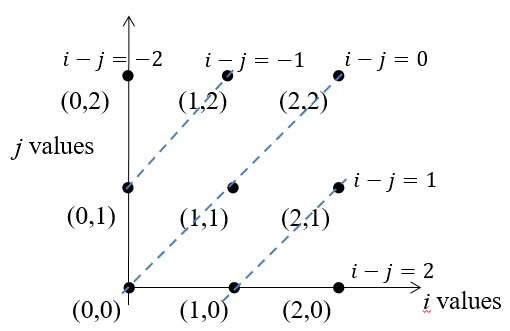
\includegraphics[width=3.0in]{images/productOfSums.png}
\caption{\label{fig:productOfSums} Grid points corresponding to the terms in the sum: $ \sum_{i=0}^{2}  \sum_{j=0}^{2} 5^{i-j} $.}
\end{center}
\end{figure} 
\end{example}

\begin{exercise}{}
By following the above argument backwards, write the following expressions as a product of sums:
\begin{enumerate}[(a)]
\item
\[\sum_{n=1}^3 n3^{3-n} + \sum_{n=1}^2 n3^{n-3}\]
\item
\[\sum_{n=1}^{10} n5^{10-n} + \sum_{n=1}^{9} n5^{n-10}\]
%\item
%\[\sum_{n=1}^3 n5^{n-1} + \sum_{n=3}^4 (5-n)5^n\]
\end{enumerate}
\end{exercise}

The situation becomes interesting when the sum inside depends on the the index variable of the outside sigma:

\[\sum_{i=0}^{3}\sum_{j=0}^{i}1\]

Unlike previous double sums, the inside sum will change depending on what $i$ is.  When $i=0$ then $\sum_{j=0}^{i}1=\sum_{j=0}^{0}1=1$ so 1 would be the first term in the outside sum.  When $i=1$ then $\sum_{j=0}^{i}1=\sum_{j=0}^{1}1=1+1=2$ so 2 would be the next term.  With each successive term, the inside sum increases by 1, so the result is $1+2+3+4 = 10$.

 Note that the index of the outer sum may appear in any or all parts of the inner sum. Here are some examples:  

\[\sum_{i=0}^{3} \sum_{j=i}^{10}1; \qquad
\sum_{i=0}^{3} \sum_{j=1}^{10i}i ; \qquad
\sum_{i=0}^{3}\sum_{j=i}^{2i}(3i+x^j).\]

In some cases, nested sums may be simplified by exchanging the order of summation.  Take for example:
\[\sum_{i=0}^{2}  \sum_{j=0}^{i}1 \]
The first term has $i=0$ and $j=0$: we write this as $(i,j)=(0,0)$. When $i=1$, then we have two terms:  $j=0$ and $j=1$. Finally, when $i=2$, we have $j=0,1,$ or 2.  Altogether we have the index pairs: $(0,0), (1,0), (1,1), (2,0), (2,1), (2,2)$. These index pairs may be displayed on a grid, as shown in Figure~\ref{fig:summation1}.
\begin{figure}[htb]
\begin{center}
	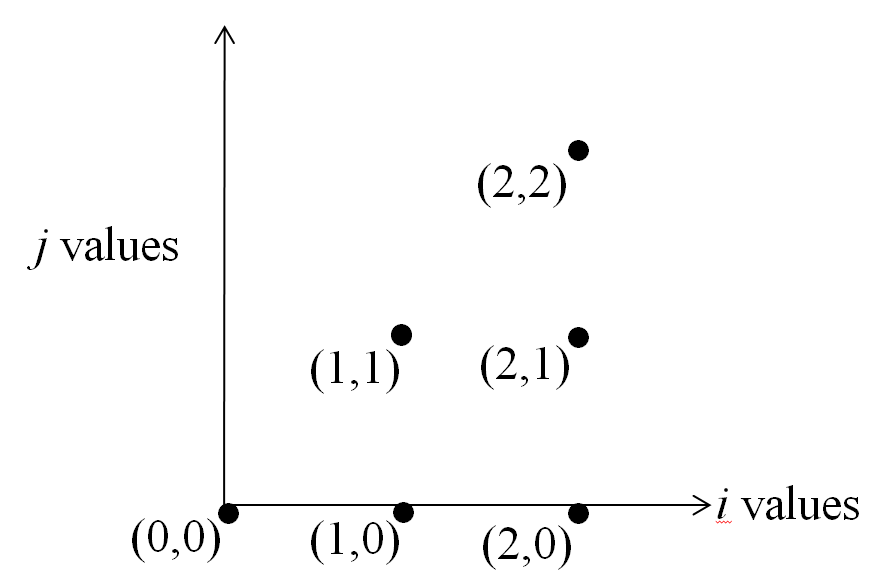
\includegraphics[width=3.0in]{images/i02j0igraph.png}
\caption{\label{fig:summation1} Grid points corresponding to the terms in the sum: $ \sum_{i=0}^{2}  \sum_{j=0}^{i}1 $.}
\end{center}
\end{figure} 

Alternatively, we can arrange these index pairs by $j$ coordinate.  When $j$ is 0, $i$ takes the values (0,1,2); when $j$ is 1, $i$ takes the values of (1,2); and when $j$ is 2, $i$ takes the value 2.  This can be expressed as the sum:
\[\sum_{j=0}^{2} \sum_{i=j}^{2}1 \]

So far our examples have only two sigmas, but it's quite possible to have an unlimited number of nested sigmas. For example, with three nested sigmas we would have grid points in three dimensions.  It doesn't matter what order you sum the terms in--as long as you include them all!

\begin{exercise}{nested1}
Draw a grid point diagram (similar to Figure~\ref{fig:summation1}) for each of the following sums.  Then use the grid point diagram  as a guide to exchanging the order of summation.
\begin{enumerate}[(a)]
\item
$\displaystyle{\sum_{i=0}^{4}\sum_{j=0}^{8}i}$
\item
$\displaystyle{\sum_{j=0}^{3} \sum_{i=j}^{j+3} (i+j)}$~~(Write as the sum of two summations.)
\item
$\displaystyle{\sum_{k=0}^{7}\sum_{i=0}^{k}(2i+1) }$
\item
$\displaystyle{\sum_{i=1}^{6}\sum_{j=i}^{i+1} (i-j) }$~~(Write as a nested sum plus two additional terms.)
\item
$\displaystyle{\sum_{i=1}^{5}\sum_{j=i}^{10} ij }$
\item
$\displaystyle{\sum_{i=m}^{n}\sum_{j=i}^{2n}jx^i }$~~(Write as the sum of two summations.)
\item
$\displaystyle{\sum_{i=m}^{n}\sum_{j=0}^{i}(i-j)^2 }$~~(You may assume $m>0$.  Write as the sum of two summations.)
\end {enumerate}
\end{exercise}

\begin{exercise}{interchangeSum}
\begin{enumerate}[(a)]
\item
Using a grid point diagram, interchange the order of summation in the following nested sum:
\[
\sum_{k=1}^{5} \sum_{\ell=1}^k (\ell + k)
\]
\item
Using a grid point diagram, interchange the order of summation in the following nested sum:
\[
\sum_{i=1}^{7} \sum_{j=1}^i ij
\]
\item
Using what you've from (a) and (b) above, give a general formula for intechanging sums of the form:
\[
\sum_{m=1}^M \sum_{n=1}^m f(m,n),
\]
where $f(m,n)$ is an arbitrary expression involving the variables $m$ and $n$.
\end{enumerate}
\end{exercise}

\begin{exercise}{}
\begin{enumerate}[(a)]
\item
In Exercise~\ref{exercise:SigmaNotation:interchangeSum}, all sums had 1 as lower limit.  Repeat the exercise (parts a,b,c) but use 0 as the lower limit on all sums.
\item
Repeat Exercise~\ref{exercise:SigmaNotation:interchangeSum} again, but use 2 as the lower limit on all sums.
\item
Based on what you have learned from (a) and (b), give a general formula for interchanging the order of summation in the following expression:
\[
\sum_{m=a}^b \sum_{n=a}^m f(m,n),
\]
\end{enumerate}
\end{exercise}


\begin{exercise}{nested2}
Using exchange of summation and other sum manipulation techniques, find the exact values of the following sums:


\begin{multicols}{2}
\begin{enumerate}[(a)]
\item
$\displaystyle{\sum_{i=1}^{9} \sum_{j=1}^{7} i(8-j)}$
\item
$\displaystyle{\sum_{i=1}^{10} \sum_{j=1}^{10} (j-i)}$
\item
$\displaystyle{\sum_{i=1}^{10} \sum_{j=1}^i \frac{1}{11-j}}$
\item
$\displaystyle{\sum_{i=1}^{10} \sum_{j=i}^{10} \frac{i}{j(j+1)}}$
\item
$\displaystyle{\sum_{i=1}^{20} \sum_{j=1}^i \frac{i}{(400-j^2)+j+20}}$ \hyperref[sec:SigmaNotation:Hints]{(*Hint*)} 
\item
$\displaystyle{\sum_{i=1}^{10} \sum_{j=1}^i (j+i)}$
\end{enumerate}
\end{multicols}
\end{exercise}

\section{Common Sums\quad
\sectionvideohref{i5RI-Ssnwps&list=PL2uooHqQ6T7PW5na4EX8rQX2WvBBdM8Qo&index=54}}
\label{sec:SigmaNotation:CommonSums}

There are several sums, even a few infinite sums, for which the total value is known. One very basic example is:
\[\sum_{i=1}^{k}1.\]

\begin{exercise}{}
Evaluate the preceding sum. Be careful-the answer is NOT 1. 
\end{exercise}

Another very useful example is:

\[\sum_{i=1}^{k}i=1+2+3\cdots+(k-1) + k\]

If one were to take the first term 1 and add it to the last term $k$, we get $k+1$.  If we take the second term 2 and add to the second-to-last term $k-1$ again we get $k+1$.  This is true for all terms in between.  In the case of an even number of terms (such as $1+2+3+4$),  the terms split evenly.  In the case of an odd number of terms (such as $1+2+3+4+5+6+7$) we have 3 pairs that add to 8 but an additional term in the middle.  In either case, we take the first term add to the last term and multiply that quantity by 1/2 the number of terms.  The formula is thus:

\[\sum_{i=1}^{k}i= \frac{k(k+1)}{2}.\] 

We can use the same reasoning to arrive at the following formula.

\[\sum_{i=a}^{k}i=a+(a+1)+(a+2)\cdots+(k-1) + k = (k+a)(k-a+1)/2,\] 
where $a$ and $k$ are integers and $a<k$.


\begin{exercise}{common1}
\begin{enumerate}[(a)]
\item 
Write the sum of odd integers from $2a+1$ to $2k+1$ in sigma notation. (Note that every odd number can be expressed as $2n+1$, where $n$ is an integer.)
\item
Give a formula for the sum that you wrote in (a).  (Use the same reasoning that we used to find sums of consecutive integers.)
\item 
Write the sum of even integers from $2a$ to $2k$ in sigma notation.
\item
Give a formula for the sum that you wrote in (c). 
\item 
Write the sum of every $5^{\text{th}}$ integer from $a$ to $a + 5k$ in sigma notation.
\item
Give a formula for the sum that you wrote in (e). 
\end {enumerate}
\end {exercise}

All of the sums in Exercise~\ref{exercise:SigmaNotation:common1} have a constant difference between consecutive terms (this constant difference is also called the \term*{step size}\index{Step size! for arithmetic sum}). The step sizes for parts (a), (c), and (e) are 2,2, and 5 respectively.  Any sum with a constant step size is called an \term{arithmetic sum}: and all arithmetic sums can be evaluated using the same technique that was used  in parts (b),(d), and (f) of the exercise.  

\term{Geometric sums} are defined as the sum of non-negative integer powers of a common base.  For example, here is a geometric sum with base 1/2:
\[
\sum_{i=0}^{n}\left({\dfrac{1}{2}}\right)^i=\left({\dfrac{1}{2}}\right)^0+\left({\dfrac{1}{2}}\right)^1+\left({\dfrac{1}{2}}\right)^2\cdots +\left({\dfrac{1}{2}}\right)^n  = 1 + {\dfrac{1}{2}} + {\dfrac{1}{4}} + {\dfrac{1}{8}}\cdots +\left({\dfrac{1}{2}}\right)^n
\]
We can evaluate this sum using an algebraic trick.  Let $S$ be the value of this sum.  We can solve for $S$  by multiplying $S$ term-by-term by 1/2 and subtracting:
\[ S=1+\frac{1}{2}+ \cdots + \frac{1}{2^n} \quad \text{and} \quad
\frac{1}{2}S=\frac{1}{2}+ \cdots + \frac{1}{2^{n+1}},
\]
so that
\[
\left(S - \frac{1}{2}S\right) = 1 - \frac{1}{2^{n+1}}.
\]
Solving this last equation for $S$ gives:
\[S=\dfrac{1 - \frac{1}{2^{n+1}}}{1-\frac{1}{2}}. \]

This same technique can be used to prove the formula for a great variety of geometric sums, as we show in the following exercise.

\begin{exercise}{geoSum}
let 
\[
S = \sum_{i=0}^{n} ar^i,
\]
where both $a$ and $r$ are complex numbers, and $n$ is a positive integer.
Use the ``sum subtraction'' technique (used above for the geometric sum with base 1/2) to derive the the following general formula:\index{Geometric series!sum of}
\[ \sum_{i=0}^{n} ar^i = a \dfrac{1-r^{n+1}}{1-r} \]
(Note the formula can also be written:  $ \sum_{i=0}^{n} ar^i = a \dfrac{r^{n+1}-1}{r-1} $.)
\end{exercise}

\begin{exercise}{}
\begin{enumerate}[(a)]
\item
Evaluate $\sum_{n=0}^{10} \left(\frac{4}{5}\right)^n$.
\item
Evaluate $\sum_{n=0}^{100} \left(\frac{4}{5}\right)^n$.
\item
Evaluate $\sum_{n=0}^{1000} \left(\frac{4}{5}\right)^n$.
\item
What do you think happen when the upper limit of the sum gets arbitrarily large?
\end{enumerate}
\end{exercise}

\begin{exercise}{}
Use ``sum subtraction'' to obtain a general formula for the following sum:
\[
S = \sum_{k=m}^{n} w\cdot z^k,
\]
Where $m,n$ are arbitrary integers ($m<n$) and $w,z$ are arbitrary nonzero complex numbers.
\end{exercise} 

\begin{exercise}{}
\begin{enumerate}[(a)]
\item
Let $z = \cis (2\pi/3)$.  Evaluate $\sum_{n=1}^3 z^n$.
\item
Let $z = \cis (2\pi/10)$.  Evaluate $\sum_{n=-4}^5 z^n$.
\item
Let $z = \cis (2\pi/13)$.  Evaluate $\sum_{n=2}^{14} z^n$.
\item
Write down an equation that generalizes the results of parts (a),(b),(c).  Prove your equation.  
\end{enumerate}
\end{exercise}


Some sums can be evaluated by grouping terms together to partially cancel out.  Two examples are:
\[
1-2+3-4+\ldots -1000 = (1-2)+(3-4)+\ldots + (999-1000)  = (-1) + (-1) + \ldots + (-1) = -500.
\]
\begin{align*}
1 - 4 + 9 -16 + 25 - 36 + \ldots +49^2 &=  1 + (-4+9) + (-16+25) + \ldots + (-48^2+49^2)\\
& = 1 + 5 + 9 + \ldots + 97\\
& = (1 + 4\cdot 0) + (1 + 4\cdot 1) + \ldots + (1 + 4 \cdot 24) \\
&= (1 + \ldots + 1) + 4\cdot(0 + 1 + \ldots + 24) \\
& = 24 + 4\cdot (24+1)\frac{24}{2}\\
&= 24 + 1200 = 1224.
\end{align*}  

In calculus you saw (or will see) sums that have an infinite number of terms, otherwise known as \term{infinite series}. Some examples include:
\begin{align*}
e^x &= \sum_{i=0}^{\infty}\dfrac{x^i}{i!} =1+\dfrac{x^1}{1!}+\dfrac{x^2}{2!}+\dfrac{x^3}{3!} \cdots \\
\sin(x) &= \sum_{i=0}^{\infty}\dfrac{(-1)^i x^{2i+1}}{(2i+1)!} = \dfrac{x^1}{1!}-\dfrac{x^3}{3!}+\dfrac{x^5}{5!}\cdots
\end{align*}

Although we won't be talking about infinite series, the same summation notation that we've been using also applies to sums with an infinite number of terms. 


\section{Summation by parts}
\label{sec:SigmaNotation:SumByParts}

Those who have studied integrals in calculus may be familiar with the process of integration by parts.  This is used when you need to find the integral of the product of two terms.  While this process is used for continuous situations, there is a version of this process for discrete situations called \term{summation by parts}.  

To show how summation by parts works, we'll look at a particular case. Consider the following product of sums:
\[\left( \sum_{n=1}^{5}a_{n} \right) \left( \sum_{n=1}^{5}b_{n} \right). \] 
If we broke this up into individual terms, we'd obtain $n \cdot n = n^2$ terms of the form $a_j b_k$.  Figure~\ref{fig:IBP}
shows the terms arranged on a grid. We've separated these terms into two parts using  a diagonal line, and we've further
grouped terms either by row (above the line) or by column (below the line). You'll see in a minute why we've arranged things like this.

\begin{figure}[htb]
\begin{center}
	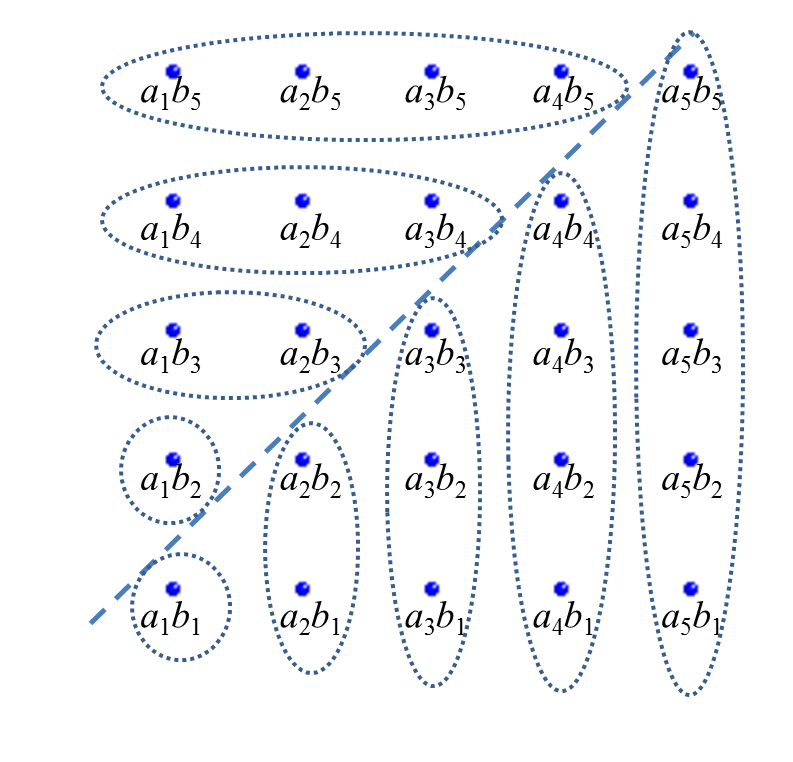
\includegraphics[width=3.0in]{images/IBP.png}
\caption{\label{fig:IBP} Arrangements of terms in the product of sums $\left( \sum_{n=1}^{5}a_{n} \right) \left( \sum_{n=1}^{5}b_{n} \right)$.}
\end{center}
\end{figure} 


Now let's go back and express the sum of all these terms a different way. We'll introduce the notation:
\[ A_{k}= \sum_{j=1}^{k}a_{j} \text{ and } B_{k}= \sum_{j=1}^{k}b_{j}. \]
$A_k$ and $B_k$ are the $k$th \term{partial sums} for the series $\sum a_j$ and $\sum b_j$, respectively.
The product of sums that we started with can be written succinctly as $A_{5}B_{5}$. 

We may use this new notation to 
re-express the grouped terms in the figure. 
Consider first the terms below the diagonal line. These terms are grouped by column, and each group is encircled by an oval:
\begin{itemize}
\item
The sum of the first oval(column on far left) is: $a_{1}b_{1}= a_{1}B_{1}$;
 \item
The sum of the second oval(column second from the left) is: $a_{2}\left ( b_{1}+b_{2} \right )= a_{2}B_{2}$;
\item
The sum the third oval(column third from the left) is: $a_{3}\left ( b_{1}+b_{2}+b_{3} \right )= a_{3}B_{3}$;
\item
The sum of the fourth oval(column fourth from left) is: $a_{4}\left ( b_{1}+b_{2}+b_{3}+b_{4} \right )= a_{4}B_{4}$;
\item 
The sum of the fifth oval(column on the far right) is: $a_{5}\left (b _{1}+b_{2}+b_{3}+b_{4}+b_{5} \right )=a _{5}B_{5}$.
\end{itemize}
Adding these five sums together accounts for all the terms below the diagonal line:
\[ a_1B_1 + a_2B_2 + \ldots + a_5B_5 = \sum_{k=1}^{5}a_kB_k,\]
where we've used summation notation to make the expression more compact.

Now let's repeat this process for the horizontal ovals above the diagonal line:
\begin{itemize}
\item
The sum for the first oval(bottom row above line) is: $a_{1}b_{2}= A_{1}b_{2}$;
\item
The sum for the second oval( second row from bottom) is: $\left ( a_{1}+a_{2} \right)b_{3}= A_{2}b_{3}$;
\item
The sum for the third oval(second row from the top) is: $\left ( a_{1}+a_{2}+a_{3} \right )b_{4}= A_{3}b_{4}$;
\item
The sum for the fourth oval(top row) is: $\left ( a_{1}+a_{2}+a_{3}+a_{4} \right)b_{5}= A_{4}b_{5}$.
\end{itemize}
Adding these five sums together accounts for all the terms below the diagonal line:
\[ A_1b_2 +  \ldots + A_4b_5 = \sum_{k=1}^{5-1}A_kb_{k+1}.\]
Since we've now accounted for terms both above and below the line, we obtain the sum of all terms by adding together:
\[ A_{5}B_{5}= \sum_{k=1}^{5}a_{k}B_{k}+\sum_{k=1}^{5-1}A_{k}b_{k+1}. \]
By rearranging this equation, we find:
\[ \sum_{k=1}^{5}a_{k}B_{k}= A_{5}B_{5}-\sum_{k=1}^{5-1}A_{k}b_{k+1}. \]

There's really nothing special about the number `5' in our above expression--we just chose it because 
this was a relatively simple case that we could illustrate. To get the general formula, we simply replace '5' with '$n$':
\[\sum_{k=1}^{n}a_{k}B_{k}= A_{n}B_{n}-\sum_{k=1}^{n-1}A_{k}b_{k+1}. \]
Notice the striking similarity between this formula and the formula for integration by parts:
\[ \int_a^b u dv =\left. uv\right|_a^b - \int_a^b v du. \] 
The resemblance makes a lot of sense, since integration is essentially a kind of summation (more precisely,
a summation taken to a limit.)

Now let's look at some examples to see how we can make use of this formula.

\begin{example}{} Evaluate $\sum_{k=1}^{n}2^{k-1}k$.
 
In order to use the summation by parts formula, we need to define $a_k$ and $B_k$ so that the summand $2^{k-1}k$ is the product of $a_k$ and $B_k$. Just as in integration by parts, we want to make our choice based on what makes the calculations easiest. 
Note that $B_{k}$  is a partial sum of $k$ terms, and that $k = 1 + \ldots + 1$. So it's natural to choose $B_{k}=k$, which means that $a_{k}=2^{k-1}$.
 
Based on our choice of $B_{k}$ and  $a_{k}$, we can now figure out $b_{k}$ and $A_{k}$.  As we noted above, $B_{k}$ is the sum of $k$ 1's, so that $b_k=1$. This leaves us with $a_k = 2^{k-1}$, so that 
\[A_{k}=\sum_{j=1}^{k}a_j.\]
 As we've seen before, we may rewrite this by shifting the starting value of the index, so that 
\[A_{k}=\sum_{j'=0}^{k-1}2^{j'} =  \frac{2^k-1}{2-1} = 2^k-1,\]
where we've used our standard formula for the sum of geometric series.

Summarizing our progress so far, we have:
\[ a_k=2^{k-1};\quad B_k=k;\quad  b_k=1; \quad A_k=2^k-1. \]
Plugging the above values into the summation by parts formula, we find:
\[ \sum_{k=1}^{n}2^{k-1}k= \left (2 ^{n}-1 \right )n-\sum_{k=1}^{n-1}\left ( 2^{k}-1 \right ). \]
The summation on the far right can be evaluated by breaking it into two separate parts:
\[ \sum_{k=1}^{n-1}\left ( 2^{k}-1 \right )= \sum_{k=1}^{n-1}2^{k}-\sum_{k=1}^{n-1}1 = (2^{n}-1)- (n-1).\]
\end{example}
We can put this into our equality and do some further algebraic puttering to obtain the final result:
\begin{align*}
\sum_{k=1}^{n}2^{k-1}k &= (2 ^{n}-1)n- (2^{n}-1)+(n-1)\\
&=  2^{n}n-n-(2^{n}-1)+(n-1)\\
&=  2^{n}n-2^{n}\\
&=  2^{n}(n-1).
\end{align*}	

\begin{exercise}{}
Evaluate $\sum_{k=1}^{n}k^{2}$ by taking $B_k=k$ and $a_k = k$. You will need the expression for the sum $1 + 2 + \ldots + m$ that we derived previously.
\end{exercise}

From the preceding examples we may see that $B_k = k$ is a frequent choice. This is closely related to the fact that $u=x$ is a frequent choice when applying  the integration by parts formula.


\begin{exercise}{}
Prove the following equation using summation by parts:
\[ \sum_{k=1}^n k^3 = \frac{n^4}{4} + \frac{n^3}{2} + \frac{n^2}{4} \]
\end{exercise}

\begin{exercise}{}
\begin{enumerate}[(a)]
\item
 Evaluate $\sum_{k=1}^{n}3^{k}k$.
\item
 Evaluate $\sum_{k=1}^{n}3^{k}k^2$.
\item
Evaluate $\sum_{k=1}^{7n} \cis(2\pi k/7)\cdot k$.
\end{enumerate}
\end{exercise}

%Example 2
%Evaluate: 
%\sum_{k=1}^{n}k^{2}
%Using our formula, we need to identify A_{l}, a_{l},  b_{l}, and B_{l} from our given summation, remembering to make choices that make calculations easiest.  At first glance, this does not appear to be a summation of a product of two amounts.  Remember, though, that k^{2}=kk. Given that both elements of the product are the same, our choice is easy and we will choose B_{l}=k and a_{l}=k.  
%By the previous example, we know that if B_{l}=k, then it follows that b_{l}=1. If a_{l}=k, then A_{l}=\sum_{l=1}^{k}a_{l}, which by substitution, A_{l}=\sum_{l=1}^{k}l which simplifies to \frac{\left ( k+1 \right )k}{2}.
%Again summarizing what we have done:
%B_{l}= k; a_{l}=k; b_{l}= 1; A_{l}= \frac{\left ( k+1 \right )k}{2}
%Plugging into the formula: \sum_{l=1}^{n}a_{l}B_{l}= A_{n}B_{n}-\sum_{l=1}^{n-1}A_{l}b_{l+1}
%\sum_{k=1}^{n}k\cdot k= \frac{n\left ( n+1 \right )n}{2}-\sum_{k=1}^{n-1}\left ( 1 \right )\frac{\left ( k+1 \right )k}{2}
%Breaking down the summation on the right,
%=\sum_{k=1}^{n-1}\left ( 1 \right )\frac{\left ( k+1 \right )k}{2}
%By factoring out \frac{1}{2}, we have the right side:
%= \frac{1}{2}\left ( \sum_{k=1}^{n-1}k^{2}+k \right )
%Breaking the summation into two parts produces:
%= \frac{1}{2}\sum_{k=1}^{n-1}k^{2}+\frac{1}{2}\sum_{k=1}^{n-1}k
%Our equation now looks like this:
%\sum_{k=1}^{n}k\cdot k= \frac{n\left ( n+1 \right )n}{2}-\frac{1}{2}\sum_{k=1}^{n-1}k^{2}-\frac{1}{2}\sum_{k=1}^{n-1}k
%Adding the summation of k^{2} to the left produces:
%\sum_{k=1}^{n}k^{2}+\frac{1}{2}\sum_{k=1}^{n-1}k^{2}= \frac{n^{2}\left ( n+1 \right )}{2}-\frac{1}{2}\sum_{k=1}^{n-1}k
%Which further simplifies on the right by replacing the summation of k with its value and separating the fraction:
%\sum_{k=1}^{n}k^{2}+\frac{1}{2}\sum_{k=1}^{n-1}k^{2}= \frac{n^{2}}{2}+\frac{n^{2}\left ( n+1 \right )}{2}-\frac{1}{2}\frac{\left ( n-1 \right )n}{2}
%Simplifying further, we can add like terms on the left (1 summation + \frac{1}{2} = \frac{3}{2}) and factor our  \frac{n}{2} on the right:
%\frac{3}{2}\sum_{k=1}^{n}k^{2}= \frac{n}{2}\left ( n+n\left ( n+1 \right )-\frac{n-1}{2} \right )
%By factoring out \frac{n}{2} on the right gives us:
%\frac{3}{2}\sum_{k=1}^{n}k^{2}= \frac{n}{2}\left ( n\left ( n+1 \right )+\frac{n+1}{2} \right )
%And finally, adding terms in the parenthesis and factoring the quadratic it produces, you are left with:
%\frac{3}{2}\sum_{k=1}^{n}k^{2}= \left ( \frac{n}{2} \right )\left ( n+1 \right )\left ( n+\frac{1}{2} \right )


\chap{Application:  Sigma Notation in Linear Algebra}{SigmaApp}

\section{Introduction to sigma notation in linear algebra\quad
\sectionvideohref{M0jHrubtHBA&list=PL2uooHqQ6T7PW5na4EX8rQX2WvBBdM8Qo&index=45}}
\label{sec:SigmaApp:LinearAlgebra}

Linear algebra is the algebra of real space: not just 3-dimensional space, but $n$-dimensional generalizations. The important mathematical objects in linear algebra are vectors and matrices: You may remember that matrices represent functions (transformations) that act  on vectors.  Although linear algebra is a relatively recent field of mathematics (which got its start in the mid-1800's), since the advent of computers it has risen to the `top of the heap' so to speak, so that  most modern applications of mathematics to real-world problems are built on linear algebra.

Sigma notation is a powerful notational tool for expressing relations and proving identities in linear algebra. In this chapter, we will look at some of the ways that sigma notation can be used to prove properties of vectors and matrices in three-dimensional space. These properties are basic to in the physics of moving objects and fields.  

This chapter ties together material from several chapters in the book. Besides sigma notation, we need concepts from sets, functions, and just a little bit from permutations (we'll give the background you need in this chapter). To understand the chapter, the reader should already have seen vectors and matrices (up to size $3\times 3$) and know a little bit about how they work.

In the following discussions, we will assume that all matrices have real entries.  However, all of the results that we will prove also apply (in some cases, with slight modifications)  for matrices with \emph{complex} entries, or matrices with entries in $\mathbb{Z}_p$.

\section{Matrix multiplication}
\label{sec:SigmaApp:MatrixMultiplication}


It should come as no surprise that summation notation commonly shows up when working with matrices. 
In the following discussion, we will follow the common practice of denoting a matrix with a capital 
letter in italics, and the entries of the matrix with the same letter in lowercase. 
Thus for example, $a_{2,4}$ denotes the entry of matrix $A$ in row 2, column 4.
   
 Consider the example of multiplying the $3 \times 3$ matrix $A$ and the $3 \times 2$ matrix $B$. 
\[{A}{B} = \left( \begin{array}{ccc}
a_{1,1} & a_{1,2}  & a_{1,3}  \\
a_{2,1} & a_{2,2} & a_{2,3} \\
a_{3,1} & a_{3,2} & a_{3,3} \end{array} \right)
 \left( \begin{array}{cc}
b_{1,1} & b_{1,2}    \\
b_{2,1} & b_{2,2}  \\
b_{3,1} & b_{3,2}  \end{array} \right) \]

\[= \left( \begin{array}{cc}
a_{1,1} b_{1,1} + a_{1,2} b_{2,1} + a_{1,3} b_{3,1} & a_{1,1} b_{1,2} + a_{1,2} b_{2,2} + a_{1,3} b_{3,2}  \\
a_{2,1} b_{1,1} + a_{2,2} b_{2,1} + a_{2,3} b_{3,1} & a_{2,1} b_{1,2} + a_{2,2} b_{2,2} + a_{2,3} b_{3,2}  \\
a_{3,1} b_{1,1} + a_{3,2} b_{2,1} + a_{3,3} b_{3,1} & a_{3,1} b_{1,2} + a_{3,2} b_{2,2} + a_{3,3} b_{3,2}  \end{array} \right) \]

Wouldn't it be nice if we could shorten that mess?  Fortunately we can!  Let the matrix ${C}$ be the product ${A} {B}$, where ${A}$ is an $m ~\times ~n$ matrix  and ${B}$ is an $n ~\times ~p$ matrix , which implies that the dimensions of ${C}$ will be $m ~ \times ~ p$.\footnote{Remember the requirement for multiplying any two matrices is that the number of columns of the first must match the number of rows of the second.}  If the row number is given by the first index (in this case $i$), and the column number is given by the second index (in this case $j$), we can write the entries of  ${C}$ as: 

\[ {c}_{i,j}= \sum_{k=1}^n a_{i,k} b_{k,j} \]


\begin{exercise}{}
In the above formula, both $i$ and $j$ are restricted to a particular range of values.  
What are the possible values of $i$ and $j$?
\end{exercise} 

Let's show how this formula works in a specific case. Suppose ${A}$ is a $3 \times 3$ matrix and ${B}$ is a $3 \times 2$ matrix as in our previous example, then the result of the product ${A} {B}$ is a $3 \times 2 $ matrix that we can call ${C}$.  Now suppose we want to find the entry on the third row in the second column of ${C}$, then we would compute:

\begin{align*}
{c}_{3,2} =& \sum_{k=1}^3 a_{3,k} b_{k,2} \\
=& a_{3,1} b_{1,2} + a_{3,2} b_{2,2} + a_{3,3} b_{3,2}.  
\end{align*}
Sure enough, when we look at the long version we wrote earlier for the product ${AB}$ our result matches the entry on the second row, third column.

The above formula makes it possible to calculate individual matrix elements, without having to compute the entire matrix.

\begin{exercise}{}
\begin{enumerate}[(a)]
\item
Let the entries of $A$ be given by $a_{i,j} = \sqrt{i+j}$ for $1 \le i,j \le 100$. Let $C = A\cdot A$ (we can also write $C=A^2$). Compute $c_{10,10}$.
\item
Let the entries of $A$ and $B$ be given by $a_{i,j} = (i+j)^2$ and $b_{i,j} = \frac{1}{i+j}$ for $1 \le i,j \le 27$. Let $C = A\cdot B$ Compute $c_{8,8}$.
\item
For the matrices $A$ and $B$ in part (b), give a general formula for $c_{k,k}, 1 \le k \le 27$ where $C=AB$.
\end{enumerate}
\end{exercise}

\begin{exercise}{}
\begin{enumerate}[(a)]
\item
Let the entries of $A$ and $B$ be given by $a_{i,j} =2^{i+j}$ and $b_{i,j} =2^{-(i+j)}$ for $1 \le i,j \le 50$. Let $C = AB$.  Compute $c_{7,11}$.
\item
Let the entries of $A$ and $B$ be given by $a_{i,j} =3^{i+j}$ and $b_{i,j} =4^{-(i+j)}$ for $1 \le i,j \le 22$. Let $C = AB$.  Compute $c_{5,4}$.
\item
Let the entries of $A$ and $B$ be given by $a_{i,j} =r^{i+j}$ and $b_{i,j} =s^{-(i+j)}$ for $1 \le i,j \le N$, where $r$ and $s$ are arbitrary real numbers. Let $C = AB$.  Give a general formula for $c_{i,j}$, $1\le i,j \le N$. (Note the same formula works if $r$ and $s$ are taken as complex numbers.) 
\end{enumerate}
\end{exercise}

\begin{exercise}{}
\begin{enumerate}[(a)]
\item
Let the entries of $A$ and $B$ be given by $a_{i,j} =2^{ij}$ and $b_{i,j} =2^{-ij}$ for $1 \le i,j \le 20$. Let $C = AB$.  Compute $c_{11,11}$.
\item
For $A,B,C$ as in part (a), compute $c_{9,6}$. 
\item
Let the entries of $A$ and $B$ be given by $a_{i,j} =2^{ij}$ and $b_{i,j} =2^{-ij}$ for $1 \le i,j \le N$. Let $C = AB$.  Give a general formula for  $c_{i,j}$ that is valid for any $(i,j)$ with $1 \le i,j \le N$.
\item
Let the entries of $A$ and $B$ be given by $a_{i,j} =w^{ij}$ and $b_{i,j} =w^{-ij}$ for $1 \le i,j \le N$, where $w$ is a fixed complex number. Let $C = AB$  Give a general formula for  $c_{i,j}$ that is valid for any $(i,j)$ with $1 \le i,j \le N$.
\end{enumerate}
\end{exercise}

\begin{exercise}{}
\begin{enumerate}[(a)]
\item
Let $z= \cis(\pi/4)$, and let the entries of $A$ and $B$ be given by $a_{i,j} =z^{ij}$ and $b_{i,j} =z^{-ij}$ for $1 \le i,j \le 8$. Let $C = AB$  Compute $c_{4,4}$ and $c_{3,5}$ .
\item
Let $z= \cis(2\pi/N)$, and let the entries of $A$ and $B$ be given by $a_{i,j} =z^{ij}$ and $b_{i,j} =z^{-ij}$ for $1 \le i,j \le N$. Let $C = AB$  Give a general formula for $c_{k,k}$ which is valid for all $k$ with $1 \le k \le N$.
\item
Let $z= \cis(2\pi/N)$, and let the entries of $A$ and $B$ be given by $a_{i,j} =z^{ij}$ and $b_{i,j} =z^{-ij}$ for $1 \le i,j \le N$. Let $C = AB$  Give a general formula for $c_{k+1,k}$ which is valid for all $k$ with $1 \le k \le N-1$.
\end{enumerate}
\end{exercise}

\begin{exercise}{sigmaAssoc}
Given three matrices $A, B, C$ with sizes $m \times n, n \times p, p \times q$ respectively.
\begin{enumerate}[(a)]
\item
Let $D = BC$.  Write a formula for the entries $d_{i,j}$ of $D$ in terms of the entries of $B$ and $C$ ($b_{i,k}$ and $c_{k,j}$, respectively). 
\item
Let $G = AD$.  Write a formula for the entries $g_{\ell,j}$ of $G$ in terms of the entries of $A$, $B$ and $C$.
\item
Let $H$ =  $(AB)$, and let $M = HC$. Write a formula for the entries $m_{\ell,j}$ of $M$ in terms of the entries of $A$, $B$ and $C$.
\item
Using parts (b) and (c), show that matrix multiplication is \emph{associative}. 
\hyperref[sec:SigmaNotation:Hints]{(*Hint*)} 
\end{enumerate}
\end{exercise}

\section{The identity matrix and the Kronecker delta}
\label{sec:SigmaApp:IdentityMatrixKroneckerDelta}

The identity matrix $I$ often comes up when working with matrices. You may remember that an identity matrix has 1's on its diagonal and 0's everywhere else:

\[I = \left[ \begin{array}{ccccc}
1 & 0  & \cdots & 0 & 0 \\
0 & 1  & \cdots & 0 & 0  \\
\vdots & \vdots & \vdots & \vdots & \vdots\\
0 & 0  & \cdots & 1 & 0  \\
0 & 0  & \cdots & 0 & 1  \\
 \end{array} \right]. \]

Notice that the ($i,j$) entry lies on the diagonal if and only if its row index ($i$) is equal to its column index ($j$).  This pattern is expressed in summation notation  by the so-called  
 \term{Kronecker delta}\index{Kronecker delta}.\footnote{After Leopold Kronecker (1823-1891), a prominent German mathematician who made many contributions to abstract algebra and number theory. Outside of those areas, he is most famous for his strong opposition to the theory of transfinite numbers first proposed by Georg Cantor (1845-1918).  Most (but not all) mathematicians today would say that Cantor was right and Kronecker was wrong. This is a fascinating research topic if you're interested in the history of mathematics.} The Kronecker delta is written as $\delta_{i,j}$ and takes the following values:

\[ \delta_{ij}=
\begin{cases}
1 ~ \text{if} ~ i=j,  \\
0 ~ \text{if} ~ i \neq j.
\end{cases} \]

By comparison with our description of the identity matrix, we may see that the $i,j$ entry of the identity matrix is equal to $\delta_{ij}$. We may denote the ($i,j$) entry of $I$ as $[I]_{i,j})$, so that:
\[  [I]_{i,j} = \delta_{ij}.\]

\begin{exercise}{KroneckerIdentity}
\begin{enumerate}[(a)]
\item
We know that if a matrix $B$ is the inverse of the $n \times n$ matrix $A$ then we have the equations: $BA = I$ and $AB = I$.  Rewrite these matrix equations in summation notation, making use of the Kronecker delta $\delta_{ij}$ (As above, denote the ($i,j$) entries of $A$ and $B$ as $a_{i,j}$ and $b_{i,j}$ respectively. You will need to choose your indices in order to make the product work out correctly.) 
\item
What matrix equation corresponds to the following system of equations in summation notation: $\displaystyle{ \sum_{k=1}^n  \delta_{ik}\delta_{kj}=\delta_{ij}}.$
\end{enumerate}
\end{exercise}

It is possible to use the Kronecker delta to define matrices besides the identity matrix. For example, consider the $4 \times 4$ matrix $A$ with entries $a_{i,j}$ defined by:
\[  a_{i,j} := \delta_{i+1,j}, \qquad 1 \le i,j \le 4.\]
In this case, the entry is 1 if the column index is one greater than the row index, and 0 otherwise:

\[A = \left[ \begin{array}{ccccc}
0 & 1   & 0 & 0 \\
0 & 0  & 1 & 0  \\
0 & 0  &  0 & 1 \\
0 & 0  & 0 & 0  \\
 \end{array} \right]. \]

\begin{exercise}{}
Write out the following   matrices:
\begin{enumerate}[(a)]
\item
The matrix $C$ defined by 
$\displaystyle  c_{i,j} := \frac{1}{2} (-\delta_{i,j+1}+\delta_{i,j-1})  \qquad 1 \le i,j \le 6$.
\item
The matrix $D$ defined by 
$\displaystyle  d_{i,j} := -2\delta_{i,j} + \delta_{i+1,j} + \delta_{i-1,j}, \qquad 1 \le i,j \le 5$.
\item 
The matrix $U$ defined by 
$\displaystyle  u_{i,j} := \delta_{i,j-1} + 2\delta_{i,j-2} + 3\delta_{i,j-3}, \qquad 1 \le i,j \le 4$.
\item
The matrix $X$ defined by 
$\displaystyle  x_{i,j} := -2\delta_{i,j} + 2\delta_{i,4-j}  \qquad 1 \le i,j \le 5$.
\end{enumerate}
\end{exercise}

For matrices that are expressable in terms of Kronecker deltas, it is possible to find matrix products using summation notation.

\begin{example}{}
Let $\mathbf{v}$ be the $10 \times 1$ matrix given by  
\[
v_{j,1} = j, j=1 \ldots 10.
\]
(Note that $\mathbf{v}$ is essentially a column vector.) Let us compute $C\mathbf{v}$, where 
the matrix $C$ defined by 
\[
  c_{i,j} := \frac{1}{2} (-\delta_{i-1,j} + \delta_{i+1,j}), \quad 1 \le i,j \le 10.
\]
The summation notation expression for the product is:
\[
[C\mathbf{v}]_{ij} = \sum_{k=1}^{10} c_{i,k} v_{k,j}.
\]
The first thing to notice is that the second index $j$ must be 1 since $\mathbf{v}$ is a $10 \times 1$ matrix. We may also substitute the expressions for $d_{i,k}$ and  $v_{k,j}$ and simplify:
\begin{align*}
[C\mathbf{v}]_{i1} &= \sum_{k=1}^{10} \frac{1}{2} (-\delta_{i-1,j} + \delta_{i+1,j}) k \qquad \qquad [\text{Definitions of } c_{i,k} \text{ and } v_{k,1}]\\ 
&= -\frac{1}{2}\sum_{k=1}^{10}  \delta_{i-1,k}k + \frac{1}{2}\sum_{k=1}^{10}  \delta_{i+1,k}k \qquad \qquad [\text{Summation rules}]
\end{align*}
At this point, we need to think about how the $\delta$'s function within these two sums. Consider the first sum, namely: 
\[ \sum_{k=1}^{10}  \delta_{i-1,k}k. \] 
For each value of $i=1,...,10$, this sum will give a different result:
\begin{itemize}
\item
When $i=1$, all terms in the sum are 0, so the result is zero.
\item
When $i=2$, the only term that contributes is the $k=1$ term, since  $\delta_{1,k} = 0$ unless $k=1$. So for $i=2$, the sum gives 1.
\item
Similarly when $i=3,...,10$, the only term that contributes is the $k=i-1$ term, since  $\delta_{3,k} = 0$ unless $k=i-1$. So the sum gives $i-1$ for $2\le i \le 10$.
\end{itemize}
We may summarize these findings as follows:
\[
\sum_{k=1}^{10}  \delta_{i-1,k}k = \begin{cases} 0 & \text{ if } i=1 \\ i-1 & \text{ if } 2 \le i \le 10. \end{cases}
\]
The second sum may be evaluated similarly: this time, $i=10$ is the exceptional case:
\[
\sum_{k=1}^{10}  \delta_{i+1,k}k = \begin{cases}  i+1 & \text{ if } 1 \le i \le 9 \\ 0 & \text{ if } i=10 . \end{cases}
\]
Substituting these expressions into our matrix product formula gives:
\[
[C\mathbf{v}]_{i1} = \begin{cases}  -\frac{0}{2} + \frac{2}{2} = 1 & \text{ if } i=1\\
							-\frac{i-1}{2} + \frac{i+1}{2} = 1 & \text{ if } 2 \le i \le 9\\
							-\frac{9}{2} + \frac{0}{2} = -4.5 & \text{ if } i=10.
                                  \end{cases}
\]
The result is a $10 \times 1$ column vector with entries all 1, except for a $-4.5$  in the $10^{\text{th}}$ entry.
\end{example}

Let's try another example, this time with two square matrices.

\begin{example}{}
This time we'll compute the entries of the matrix product $FV$, where the entries $f_{ij}$ of $F$ and $v_{ij}$ of $V$ are given by:
\[
f_{ij} := \delta_{i+1,j} - \delta_{i,j}; \qquad v_{i,j} := 2^{i+j}, \quad 1 \le i,j \le 20.
\]
We may begin once again with the matrix product formula:
\begin{align*}
[FV_{ij} &= \sum_{k=1}^{20} f_{ik}v_{kj} \qquad \qquad [\text{Matrix mulitplication formula }]\\ 
&=  \sum_{k=1}^{20} (\delta_{i+1,k} - \delta_{i,k})2^{k+j} \qquad \qquad [\text{Substitution}]\\
&=  \sum_{k=1}^{20} \delta_{i+1,k}2^{k+j} - \delta_{i,k}2^{k+j} \qquad \qquad [\text{Substitution}]\\
&= 2^{i+1+j} - 2^{i+j} \qquad \qquad [\text{Select nonzero term in each summation}]\\
&= 2^{i+j}(2 - 1) \qquad \qquad [\text{Factor out common factor}]\\
&= 2^{i+j}. \qquad \qquad \qquad [\text{Exponent rules}]\\
\end{align*}

The shakiest step in this computation is the one labeled ``Select nonzero term in each summation'', and we should double-check to make sure we did it right.  When $i = 1,2,...,19$, then it is always true that 
$\delta_{i+1,k}$ will be nonzero for a single value of $k$ between 1 and 20, so the sum over $k$ of $\delta_{i+1,k}$ will reduce to a single term. But the case $i=20$ is different.  In this case, $\delta_{20+1,k}$ is equal to 0 for \emph{all} values of $k$ between 1 and 20. So we'll have to redo the calculation in this case:
\begin{align*}
\sum_{k=1}^{20} \delta_{20+1,k}2^{k+j} - \delta_{20,k}2^{k+j} &= 0 - 2^{2-+j}\\
&= - 2^{20+j}.
\end{align*}
This brings us to the final result: 
\[
[FV]_{ij} = \begin{cases}  2^{i+j} & \text{ if } 1 \le i \le 19 \text{ and } 1 \le j \le 20\\
					- 2^{20+j}	  & \text{ if } i=20 \text{ and } 1 \le j \le 20.\\
                   \end{cases}
\]
 \end{example}

\begin{exercise}{}
Let $\mathbf{v}$ be the $10 \times 1$ matrix (a.k.a column vector) given by:  $v_{j,1} = j^2,$ $j=1 \ldots 10$. Compute $D\mathbf{v}$, where 
the entries of $D$ are given by 
$\displaystyle  d_{i,j} := -2\delta_{i,j} + \delta_{i+1,j} + \delta_{i-1,j}, \qquad 1 \le i,j \le 10$
(The matrix $D$ is an example of a \term{discrete second derivative matrix}\index{Matrix!discrete second deriviatve}.)
\end{exercise}

\begin{exercise}{}
Let $F$ and $B$ be the $50 \times 50$ matrices defined by  $f{i,j} = \delta_{i+1,j} - \delta_{i,j}$, and $b_{i,j} = \delta_{i,j}-\delta_{i-1,j}$, respectively.  ( $F$ and $B$ are examples of  \term{forward difference matrix} and \term{backward difference matrix}, respectively.)\index{Matrix!forward difference}\index{Matrix!backward difference}
\begin{enumerate}[(a)]
\item
Compute $FB$.
Compute $BF$. 
\end{enumerate}
\end{exercise}


It turns out that matrices defined using Kronecker deltas play a prominent role in numerical analysis, and in particular the numerical solution of ordinary and partial differential equations.

\section{Abbreviated matrix notations}
\label{sec:SigmaApp:AbbrevMatrixNotations}

In the following discussion, we will be seeing lots of sums involving matrices. This being the case, it's worth our while to try to simplify our notation. In our expression for $C=AB$, we had:
\[ {c}_{i,j}= \sum_{k=1}^n a_{i,k} b_{k,j} \]
Now, notice that the index $k$ runs over all columns of $A$ and all rows of $B$  (recall that matrix multiplication is only defined if the number of columns of $A$ is equal to the number of rows of $B$). This being the case, we don't really need to mention that $k$ runs from 1 to $n$--we should simply understand that the index $k$ runs over all possible values. We can therefore convey the same information by simply writing:
\[ {c}_{i,j}= \sum_{k} a_{i,k} b_{k,j}. \]
This makes more complicated matrix multiplications much simpler. For example, if $D = (AB)C$ where $A$ is $n \times p$, $B$ is $p \times q$, and $C$ is $q \times r$ instead of
\[ {d}_{i,m}= \sum_{j=1}^q \left( \sum_{k=1}^p a_{i,k} b_{k,j} \right) c_{j,m}, \]
 we may write
\[ {d}_{i,m}= \sum_{j} \left( \sum_{k} a_{i,k} b_{k,j} \right) c_{j,m}, \]
which further simplifies to
\[ {d}_{i,m}= \sum_{j,k}  a_{i,k} b_{k,j} c_{j,m}. \]
We could write either $\sum_{j,k}$ or $\sum_{k,j}$:  all possible values of $k$ and $j$ are summed over, so it doesn't matter which order we mention the indices.

There is an even more abbreviated notation that is commonly used in physics, called \term{Einstein notation}  (yes, it's that Einstein!) Notice that in our expression for ${c}_{i,j}$, the subscript $k$ is \emph{repeated}: that is, it appears as a subscript on $a_{i,k}$ and on  $b_{k,j}$. Similarly, in our expression for ${d}_{i,m}$  the summed subscripts ($j$ and $k$) are also repeated: both appear as subscripts in two terms. The Einstein rule may be summarized as:
\[ \text{Repeated indices are assumed to be summed.} \] 
So for example, the expression
\[ {d}_{i,m}= \sum_{j} \left( \sum_{k} a_{i,k} b_{k,j} \right) c_{j,m} \]
in  Einstein notation simplifies to:
\[ {d}_{i,m}=  a_{i,k} b_{k,j} c_{j,m}. \]

\begin{exercise}{abbreviated1}
Write the following expressions in both abbreviated notations. Note that all indices are summed over the full range of possible values.
\begin{enumerate}[(a)]
\item
$\sum_{i=1}^m \left( \sum_{j=1}^n \left( \sum_{k=1}^p  a_{i,j} b_{j,i} \right) c_{k,k}\right)$
\item
$\sum_{\ell=1}^L \left( \sum_{m=1}^M \left( \sum_{n=1}^N  a_{\ell,m} b_{n,\ell} \right) c_{m,n} \right)$
\end{enumerate}
\end{exercise}

\begin{exercise}{unabbreviated1}
Suppose $A,B,C,D$ are $n \times n$ matrices.  Write the complete (unabbreviated) expression corresponding to the following sums in Einstein notation:
\begin{enumerate}[(a)]
\item
$a_{i,j}a_{k,\ell}b_{p,k}b_{i,\ell}$
\item
$d_{i,j}a_{k,\ell}b_{j,k}b_{i,\ell}$
\end{enumerate}
\end{exercise}

In the following sections we will use the first type of abbreviated notation (not Einstein notation).


\section{Matrix transpose and matrix inverse}
\label{sec:SigmaApp:MatrixTransposeInverses}

\subsection{Matrix transpose}
\label{subsec:SigmaApp:MatrixTransposeInverses:MatrixTranspose}

Transpose is another operation on matrices that lends itself to summation notation.  Recall that the transpose of a matrix changes the rows to columns,so that the first row becomes the first column, the second row becomes the second column, and so on.  The transpose of matrix $A$ is denoted as $A^{\text{T}}$.\index{Transpose!of a matrix}\index{Matrix!transpose} Using indices and recalling that first index is the row and the second is the column, we can express this as:

\[ \left[ {A}^{\text{T}} \right]_{i,j} = \left[ A \right]_{j,i}, \]
that is, the $(i,j)$ entry of $A^{\text{T}}$ is equal to the $(j,i)$ entry of $A$.  Since we typically write the $(j,i)$ entry of $A$ as $a_{j,i}$, we may also write:
\[ \left[ {A}^{\text{T}} \right]_{i,j} = a_{j,i}. \]
Don't get caught up with the particular indices $i$ and $j$--the important thing is that the indices are switched when you take the transpose.  For example, we can also write $\left[ {A}^{\text{T}} \right]_{j,i} = a_{i,j}$ or 
$\left[ {A}^{\text{T}} \right]_{k,m} = a_{m,k}$.

Now let's demonstrate the power of our new notation to prove an important property of transpose:

\begin{prop}{prodTrans}
If $A$ and $B$ are matrices such that the matrix product is defined, then 
\[ \left( {A}{B} \right)^{\text{T}} = {B}^{\text{T}} {A}^{\text{T}}. \]
\end{prop}


\begin{proof}
We'll prove this by expressing the $(i,j)$ entry of the left-hand side in summation notation,  doing some algebraic hocus-pocus, and showing that it agrees with the $(i,j)$ entry of the right side.  First we make things clear by specifying that ${A}$ has $n$ columns and $B$ has $n$ rows (these dimensions have to agree, or the product is not defined). This gives us
\[ \left[ AB \right]_{i,j}= \sum_{k} a_{i,k} b_{k,j}. \]
(remember that we decided to use abbreviated notation, so we leave off the summation limits) so the $(i,j)$ entry of the left-hand side is:
 \[ \left[ (AB)^T \right]_{i,j} = \left[ AB \right]_{j,i} = \sum_{k} a_{j,k} b_{k,i}. \]

At this point we can introduce ${A}$ and ${B}$ transpose  because the $j,k$ entry of any matrix is the $k,j$ entry of its transpose:

\[  \sum_{k} a_{j,k} b_{k,i} =  \sum_{k} \left[A^{\text{T}}\right]_{k,j} \left[B^{\text{T}}\right]_{i,k.} \]

Since the terms of ${A}$ and ${B}$ are being expressed as a summation, they commute (i.e. order doesn't matter), which allows us to say (using our definition of matrix product):

\[ \sum_{k} \left[A^{\text{T}}\right]_{k,j} \left[B^{\text{T}}\right]_{i,k} = \sum_{k} \left[B^{\text{T}}\right]_{i,k}\left[A^{\text{T}}\right]_{k,j} = \left[ {B}^{\text{T}}{A}^{\text{T}} \right]_{i,j}, \]

Voil\`{a}, we have the $(i,j)$ entry of the right-hand side, and the proof is complete.
\end{proof}


\begin{exercise}{}
Give a formula for $(ABC)^T$, and prove your formula using summation notation.
\end{exercise}

\begin{exercise}{}
We know that the transpose of a $n \times n$ matrix is a $n \times n$ matrix.  So we can consider transpose as a function from $M_n(\mathbb{R})$ to $M_n(\mathbb{R})$, where   $M_n(\mathbb{R})$  is the set of $n \times n$ matrices with real-number entries. Prove or disprove the following:
\begin{enumerate}[(a)]
\item
Transpose defines an invertible function from $M_n(\mathbb{R})$ to $M_n(\mathbb{R})$.
\item
Transpose preserves addition, i.e. $A^T + B^T = (A+B)^T$ for any matrices $A,B \in M_n(\mathbb{R})$.
\item
Transpose preserves multiplication, i.e. $A^T \cdot B^T = (A\cdot B)^T$ for any matrices $A,B \in M_n(\mathbb{R})$.

\end{enumerate}
\end{exercise}



\subsection{Matrix inverse}
\label{subsec:SigmaApp:MatrixTransposeInverses:MatrixInverse}

We can also express matrix inverse equations in summation notation.  Recall that the inverse of a matrix $A$ is a matrix $A^{-1}$ such that $AA^{-1}=I$ and $A^{-1}A=I$.

\begin{exercise}{inverse1}
\begin{enumerate}[(a)]
\item
Express the equations $AA^{-1}=I$ and $A^{-1}A=I$ using summation notation.  You may use the notation $[A]_{i,j}$ and $[A^{-1}]_{i,j}$ to express the entries of the two matrices.
\item
Suppose that $A$ and $B$ are invertible square matrices of the same size (so that $A^{-1}$ and $B^{-1}$ exist and are also of the same size). Prove that $(AB)^{-1} = B^{-1}A^{-1}$.
\end{enumerate}
\end{exercise}

\section{Rotation matrices (in 3 dimensions)}
\label{sec:SigmaApp:RotationMatrix3D}


In three-dimensional space, the \term{dot product} (or \term{scalar product}) of two vectors $v:=[v_1,v_2,v_3]^{\text{T}}$ and $w:=[w_1,w_2,w_3]^{\text{T}}$ is defined as
\[ v \cdot w :=  v_1w_1 + v_2w_2 + v_3w_3 = \sum_j v_j w_j ,\]
where we have made use of summation notation to shorten the expression. If we also define the \term*{length}\index{Length!of a vector} of the vector $v$ (denoted by $||v||$) as
\[ \lVert v\rVert := (v \cdot v)^{1/2}, \]
then we may then write the \term{cosine formula} as
\[ \cos(\theta) = \frac{v \cdot w}{\lVert v \rVert \lVert w \rVert}, \]
where $\theta$ is the angle between the two vectors $v$ and $w$. (You may have encountered this formula in physics class or precalculus.)

Any $3 \times 3$ matrix $A$  produces a function from three-dimensional space to itself as follows: given any vector $v:=[v_1,v_2,v_3]^{\text{T}}$, then the image vector is $Av$. Using summation notation, we may write:
\[ [Av]_i = \sum_j A_{ij} v_j.\]
A matrix is called a \term{rotation matrix} if it satisfies the following properties:
\begin{itemize}
\item
A rotation matrix $R$ must  \emph{preserve  lengths and angles}. In other words, if $v$ and $w$ are any two 3-d vectors , then  $\lVert Rv \rVert = \lVert v \rVert$,  $\lVert Rw \rVert = \lVert v \rVert$, and furthermore the angle between $Rv$ and $Rw$ must be the same as the angle between $v$ and $w$.  In view of the cosine formula, this means that the dot product must be preserved:  $Rv \cdot Rw = v \cdot w$. In fact, since vector length is the square root of a dot product, all of these conditions will be satisfied as long as 
\[ Rv \cdot Rw = v \cdot w \] 
for any two 3-d vectors $v$ and $w$.
\item
A rotation matrix must \emph{preserve handedness}. This means that if the vectors $\{ [1,0,0]^{\text{T}}, [0,1,0]^{\text{T}}, [0,0,1]^{\text{T}} \}$ form a right-handed coordinate system, then the image vectors 
$\{ R[1,0,0]^{\text{T}}, R[0,1,0]^{\text{T}}, R[0,0,1]^{\text{T}} \}$ must also form a right-handed coordinate system.  
\end{itemize}

It turns out that this second condition implies that $\det(R)\ge 0$. We won't prove this, but we can give a few examples to show that it is reasonable. Consider  the $3 \times 3$ matrix $-I$, which has determinant equal to $-1$. This matrix will map the $x$, $y$, and $z$ axes to the $-x$, $-y$, and $-z$ axes respectively. By using the right-hand rule, you may verify that if the $x$, $y$, and $z$ axes form a right-handed coordinate system, then the $-x$, $-y$, and $-z$ axes form a left-handed coordinate system.

The following exercise gives some other examples of matrices $R$ with $\det(R)< 0$ which do not preserve handedness.

\begin{exercise}{}
\begin{enumerate}[(a)]
\item
Find a matrix which  maps the $x$, $y$, and $z$ axes to the $-x$, $y$, and $z$ axes respectively.  What's its determinant?
\item  show that the function defined in (a) maps a right-handed coordinate system to a left-handed coordinate system.
\item Repeat parts (a) and (b) for the case where the $x$, $y$, and $z$ axes to the $x$, $-y$, and $z$ axes respectively.
\end{enumerate}
\end{exercise}

So let's go back to the first condition for rotation matrices, namely that they preserve inner products: $Rv \cdot Rw = v \cdot w$. Let's rewrite this in coordinate notation. First, note that $[Rv]_k$  and $[Rw]_k$ can be written as $\sum_i r_{ki}v_i$ and $\sum_j r_{kj} w_j$ respectively, where $r_{kj}$ is  the $(k,j)$ entry of $R$. Therefore we have:
\begin{align*}
 Rv \cdot Rw &= \sum_k  [Rv]_k[Rw]_k \\
&= \sum_k \left(\sum_i r_{ki}v_i \right)\left(\sum_j r_{kj}w_j \right)] \\
&= \sum_{i,j,k} (r_{ki}v_i)(r_{kj}w_j) \\
&= \sum_{i,j,k} r_{ki}r_{kj} v_i w_j. 
\end{align*}
Recall our rotation condition:  $ Rv \cdot Rw = v\cdot w$, which must be true for any two vectors $v$ and $w$. In summation notation, this becomes:
\[\sum_{i,j,k} r_{ki}r_{kj} v_i w_j =  \sum_m  v_m w_m \]
Now let's consider different possibilities for $v$ and $w$. For example we may let $ v=w=[1,0,0]^{\text{T}}$. this means that $v_i = \delta_{i1}$ and $w_j = \delta_{j1}$, where $\delta$ is our old friend the Kronecker delta.  Plugging this into our summation notation expression gives:
\[\sum_{i,j,k} r_{ki}r_{kj} \delta_{i1}\delta_{j1} =  \sum_m  \delta_{m1}\delta_{m1}. \]
Because of the $\delta$'s, when we sum over $i,j$, and $m$ the only terms that contribute will be $i=j=m=1$.  In summary, we obtain:
\[\sum_{k} r_{k1}r_{k1}  = 1. \]
Using this strategy, we can obtain a whole bunch of identities:

\begin{exercise}{}
\begin{enumerate}[(a)]
\item
By plugging in different possibilities for $v$ and $w$, show that if
\[\sum_{i,j,k} r_{ki}r_{kj} v_i w_j =  \sum_m  v_m w_m \]
holds for all $v, w$ then 
\[\sum_{k} r_{ki}r_{kj}  = \delta_{ij}. \]
\item
Show the converse of (a), namely:  given that
\[\sum_{k} r_{ki}r_{kj}  = \delta_{ij}, \]
show that
\[\sum_{i,j,k} r_{ki}r_{kj} v_i w_j =  \sum_m  v_m w_m \]
for all $v, w$.
\item
Show that the expression $\sum_{k} r_{ki}r_{kj}  = \delta_{ij}$ can be rewritten in matrix form as:
\[R^{\text{T}}R = I.\]
\end{enumerate}
\end{exercise}
We summarize these results in a proposition:

\begin{prop}{rotTrans} A $3 \times 3$ matrix $R$ is a rotation matrix if and only if $\det(R)>0$ and $R^{\text{T}}R = I$.
\end{prop}
We will pick up on rotation matrices in Section~\ref{subsec:SigmaApp:LeviCivitaAndApp:LeviCivitaDet} when we talk about determinants, and again in Section~\ref{subsec:SigmaApp:LeviCivitaAndApp:EulerRot} when we prove Euler's rotation theorem.

\section{Matrix traces}
\label{sec:SigmaApp:MatrixTraces}

Another cool application of summation notation with matrices is to prove things about the \term{trace}\index{Trace!of a matrix} of a matrix.  The trace only applies to square matrices (equal number of rows and columns) and is the sum of all the entries on the diagonal--that is,  the sum of all entries with the same column and row number.  In summation notation, the trace of an $n \times n$ matrix as:

\[ \text{Tr} \left( A \right)= a_{1,1} + a_{2,2} + \ldots + a_{n,n} = \sum_{i} a_{i,i} \] 
This time we are using the index $i$ for both the row position and the column position, so its the position of the index that denotes row and column.  The formula for the product used two different letters for the indices because they were not always equal, but for trace the row and column number will always be equal, so we only need one letter.

The next exercise covers some basic properties of traces:

\begin{exercise}{trace1}
\begin{enumerate}[(a)]
\item
Prove that if $A$ and $B$ are square matrices of the same size, then $\text{Tr} \left( A + B \right) = \text{Tr} \left( A \right) + \text{Tr} \left( B \right)$.
\item
Prove that if $A$ is a square matrix with real entries and $k$ is a real number, then $\text{Tr} \left(k A  \right) = k\text{Tr} \left( A \right)$.
\end{enumerate}
\end{exercise}


In the above exercise, we have considered the trace of the sum of two matrices. Now we consider the trace of the \emph{product} of two matrices.  To this end, let ${A}$ and  ${B}$ be a $n \times n$ matrices.  So first we have:

\[ \text{Tr} \left({A} {B}\right) = \sum_{i} [AB]_{i,i} = \sum_{i}\left( \sum_k a_{i,k}b_{k,i}\right) = \sum_{i,k}a_{i,k}b_{k,i}. \]

All we've done here is take the matrix product formula, and set the second index of the second  matrix entry equal to first index of the first matrix entry.  Now to make things interesting, let's find the trace for the reverse order:

\[ \text{Tr} \left({B} {A}\right) = \sum_{i} [BA]_{i,i} = \sum_{i} \left( \sum_{k} b_{i,k}a_{k,i} \right) = \sum_{i,k}a_{k,i}b_{i,k}. \]

Let's play with this last equation a bit. As we mentioned before, we can change the sum over $i,k$ to a sum over $i,k$ without changing anything. Furthermore, since $b_{i,k}$ and $a_{k,i}$ are numbers, they commute under multiplication:

\[ \text{Tr} \left({B} {A}\right) =\sum_{i,k} b_{i,k}a_{k,i} =  \sum_{k,i} a_{k,i}b_{i,k}. \]

Finally, we rename the indices by changing $k$ to $i$ and $i$ to $k$.  (Remember, it's the positions of the indices that are important, not the letters we call them by!)  After renaming, we get:

\[ \text{Tr} \left({B} {A}\right) =\sum_{i,k} a_{i,k}b_{k,i}, \]

which agrees with our original expression for  $\text{Tr} ({A}{B})$.

\begin{exercise}{}
In the above proof that $\text{Tr} ({AB}) = \text{Tr}({BA})$, we assumed that both $A$ and $B$ were square matrices. Show that the formula is still true when $A$ is a $m \times n$ matrix and $B$ is a $n \times m$ matrix.  (Notice that $AB$ and $BA$ are both square matrices, so that $\text{Tr} \left({A} {B}\right)$ and $\text{Tr} \left({B} {A}\right)$ are both well-defined.)
\end{exercise}

\begin{exercise}{trace3}
Show that $\text{Tr} ({ABC}) = \text{Tr}({CAB})$, as long as the dimensions of $A, B, C$ are such that the products are well-defined.
\hyperref[sec:SigmaNotation:Hints]{(*Hint*)} 
\end{exercise}


\begin{exercise}{}
Show that 
\[ \text{Tr} ({ABCD}) = \text{Tr}({DABC})= \text{Tr}({CDAB}) = \text{Tr}({BCDA}),\] 
as long as the matrices have dimensions so that all of these products are defined.  Notice that all of these arrangements of the matrices $A, B, C, D$ are \emph{cyclic permutations} of each other.
\end{exercise}

\begin{exercise}{linalg}
In linear algebra, given two $n \times n$ matrices $A$ and $B$ we say that $A$ is \term{similar}\index{Matrices!similar} to $B$ if there exists an invertible matrix $S$ such that $B = S^{-1}AS$. 
\begin{enumerate}[(a)]
\item
Prove that if $A$ is similar to $B$, then $B$ is similar to $A$.
\hyperref[sec:SigmaNotation:Hints]{(*Hint*)} 
\item
Prove that if $A$ is similar to $B$, then $\text{Tr} ({A}) = \text{Tr} ({B})$. 
\hyperref[sec:SigmaNotation:Hints]{(*Hint*)} 
\end{enumerate}
\end{exercise}

\begin{exercise}{}
Let $A$ be a $n \times n$ diagonal matrix with positive entries, so that the entries of $A$ are given by:  $ [A]_{i,j} = a_{i} \delta_{ij}$ where $a_i > 0, i = 1, \ldots, n$.  Define the matrix $\log A$ as follows:  $ [\log A]_{i,j} = \log(a_{i}) \delta_{ij}$, where $\log$ refers to natural logarithm.  Show that:

\[ \text{Tr}(\log A) = \log (\det A). \]
(Remember that the determinant of a diagonal matrix is the product of the entries on the diagonal.)
This formula is actually quite general, and applies to many non-diagonal matrices as well, as long as $\log A$ is properly defined. \footnote{In some cases, the formula can be used to estimate the determinants of very large matrices: see \url{http://arxiv.org/pdf/hep-lat/9707001}.} 
\end{exercise}

%%% This problem is an orphan that needs a good home.


\section{Levi-Civita symbols and applications}
\label{sec:SigmaApp:LeviCivitaAndApp}

\subsection{Levi-Civita symbols: definitions and examples}
\label{subsec:SigmaApp:LeviCivitaAndApp:LeviCivita}

When dealing with vectors and matrices in physics, one often finds lurking  the Levi-Civita symbol,\footnote{Levi-Civita actually refers to one person, not two: the Italian mathematician Tullio Levi-Civita, (1873-1941), who worked on mathematical physics (including relativity).} which is written as an epsilon (the Greek letter $\epsilon$) with various numbers of subscripts.  The possible values it can take are 1, -1, or 0, depending on the values of the subscripts (we refer to these subscripts as ``indices'').  This might not seem too useful since it can only take three different values, but you will see that it does a great job of simplifying expressions that ordinarily would be much more complicated.  

For an epsilon with two indices (written as $\epsilon_{ij}$), each index can be either 1 or 2. The different values that $\epsilon_{ij}$ can take are:

\[ \epsilon_{ij}=
\begin{cases}
\,\,1 ~ \text{if} ~ i=1, j=2,  \\
-1 ~ \text{if} ~ i=2, j=1,  \\
\,\, 0 ~ \text{if} ~ i=j.
\end{cases} \]

For an epsilon with three indices, each index can be either 1,2,or 3. The values of $\epsilon_{ijk}$ are:

\[ \epsilon_{ijk}=
\begin{cases}
1 ~ \text{where} ~ (i,j,k)= (1,2,3),  (2,3,1),  \mathrm{~or~}(3,1,2), \\
-1 ~ \text{where} ~ (i,j,k) = (2,1,3), (1,3,2),  \mathrm{~or~}(3,2,1),  \\
0 ~ \text{where} ~  i=j, i=k, ~ \text{or} ~ j=k, ~ \text{i.e., if any index is repeated.}
\end{cases} \]

What's the rule behind this definition?  
The six possible rearrangements of $(1,2,3)$ in the definition of $\epsilon_{ijk}$ are called \emph{permutations}\index{Permutation}.  
The three arrangements $(2,1,3)$, $(1,3,2)$, and $(3,2,1)$  can all be obtained from $(1,2,3)$ by a single exchange of two numbers.  For example, $(2,1,3)$ is obtained from $(1,2,3)$ by exchanging $1 \leftrightarrow 2$; and the other two rearrangements exchange $2 \leftrightarrow 3$ and $1 \leftrightarrow 3$ respectively.  On the other hand, to get $(2,3,1)$ or $(3,1,2)$ from $(1,2,3)$ requires \emph{two} exchanges.  Since the number of exchanges for $(2,1,3), (1,3,2), and (3,2,1)$ is odd, these are called \emph{odd permutations}\index{Permutation!odd and even}, while the others (including $(1,2,3)$  are called \emph{even  permutations}.   So the definition of   $\epsilon_{ijk}$ may be summarized as follows:  it's equal to 1 if $(i,j,k)$ is an even permutation, $-1$ if  $(i,j,k)$ is an odd permutation, and 0 if $(i,j,k)$ is not a permutation (i.e. there are repeated indices.

You may wonder, Why this strange definition?  We'll see more reasons later, but for now we can relate the definition of  $\epsilon_{ijk}$  to rotations of the $x,y,z$ axes in 3-dimensional space. Let's call these axes 1,2,3 instead of $x,y,z$ Now, if it is possible to rotate the axes so that 1 moves to 2, 2 moves to 3, and 3 moves to 1: in other words $(1,2,3)$ has moved to $(2,3,1)$. It's also possible to move $(1,2,3)$ to $(3,1,2)$.  Notice that these two  are exactly the even permutations!  On the other hand, it is not possible to move $(1,2,3)$ to $(1,3,2)$:  To do so would require turning one of the axes around  (this is called a \emph{reflection}\index{Reflection}). So the sign of   $\epsilon_{ijk}$  distinguishes rotations from reflections. Besides this geometrical interpretation, we'll have a lot more to say about even and odd permutations in Section~\ref{sec:Permutations:OtherGroups}.)  

We may simplify the notation somewhat if we define the \term*{sign} of a permutation as follows:

\[ \text{sign}(\sigma)=
\begin{cases}
1 \quad \text{if } \sigma \text{ is an even permutation,}\\
-1 \quad \text{if } \sigma \text{ is an even permutation.}
\end{cases} \]

We may then concisely express the general definition  of the \term{Levi-Civita symbol} with $n$ indices as:

\[ \epsilon_{i_1 i_2 i_3 \ldots i_n}=
\begin{cases}
\text{sign} \left( \begin{smallmatrix} 1&2&3&\ldots&n \\ i_1&i_2&i_3 &\ldots&i_n \end{smallmatrix} \right) \text{if no indices are repeated,}\\
0 ~ \text{if any  index is repeated.}
\end{cases} \]

The symbol with $n$ indices is sometimes called an $n$-dimensional Levi-Civita symbol: for instance, $\epsilon_{ijk}$ is a 3-dimensional Levi-Civita symbol.  The reason for this is that most often they are used with vector spaces that have the same dimension as the number of indices in the symbol.  So   the Levi-Civita symbol with three indices, $\epsilon_{ijk}$ is most useful in three dimensions, as we'll see shortly.

\begin{exercise}{KLC}
Using  the general definition of the Levi-Civita symbol, show that:
\begin{enumerate}[(a)]
\item
$\displaystyle \sum_{i,j} \epsilon_{ij} \delta_{ij}=0$
\item
$ \epsilon_{i_1i_2\ldots i_n} \delta_{i_ji_k}=0$ for any $j,k$ such that $1 \le j < k \le n$,
\item
$\epsilon_{ijk} = \epsilon_{jki} = \epsilon_{kij}.$
\end{enumerate}
\end{exercise}

In the Set Theory chapter you saw the formula:
\[ |A \cup B| = |A| + |B| - |A \cap B|.\]
This means that you may count all the elements contained in set $A$ or set $B$ by counting the elements in $A$ and $B$ separately, then subtracting their intersection.  You have to  subtract the intersection because  the overlap between $A$ and $B$ gets counted twice in the separate counts of $A$ and $B$.  (Think of a set diagram, where $A$ and $B$ are represented by intersecting circles.)  When we split up summations depending on whether indices are equal or unequal, we have to add and subtract in a similar way. We can prove this using Levi-Civita symbols.
  
\begin{exercise}{split}
\begin{enumerate}[(a)]
\item
Show that for any values $i,j,k \in \{1,2,3\}$, it is always true that 
\[ 1=|\epsilon_{ijk}|+\delta_{ij}+\delta_{jk}+\delta_{ik}-2\delta_{ij}\delta_{ik}\]
 \hyperref[sec:SigmaNotation:Hints]{(*Hint*)}.   
\item
Show that 
\[
\sum_{i,j,k} a_{i,j,k}=\sum_{i,j,k~\text{all unequal}}a_{i,j,k}+\sum_{i,k}a_{i,i,k}+\sum_{i,j}a_{i,j,j}+\sum_{j,k}a_{k,j,k}-2\sum_{i}a_{i,i,i}.
\]
\hyperref[sec:SigmaNotation:Hints]{(*Hint*)} 
\end{enumerate}
\end{exercise}


\subsection{Levi-Civita symbols and determinants}
\label{subsec:SigmaApp:LeviCivitaAndApp:LeviCivitaDet} 

Now that we've defined Levi-Civita symbols, we can actually use them for something!  The first application we'll look at is determinants.  Suppose you have a $2 \times 2 $ matrix $A$:

\[ A = \left( \begin{array}{cc}
a_{11} & a_{12} \\
a_{21} & a_{22} \end{array} \right) \]
\noindent
(Note that previously we separated multiple subscripts with a comma, e.g. $a_{i,j}$: but from now on we'll leave out the comma (e.g. $a_{ij}$), which is the way most math books do it.)

Then the determinant is:

\[ \text{det} (A) = 
 \left| \begin{array}{cc} a_{11} & a_{12} \\
a_{21} & a_{22} \end{array} \right|
= a_{11}a_{22} - a_{12}a_{21} \]

We can write this using the Levi-Civita symbol as:

\[ \text{det} A = \sum_{i,j} \epsilon_{ij} a_{1i} a_{2j} \]

Let's check this by evaluating the double sum. Remember that in this case, both $i$ and $j$ run from 1 to 2
\begin{align*}
\text{det} A =& \sum_{i,j} \epsilon_{ij} a_{1i} a_{2j} \\
=& \sum_{i} \left( \sum_{j} \epsilon_{ij} a_{1i} a_{2j}\right) \\
=& \sum_{i} \left( \epsilon_{i1} a_{1i} a_{21} + \epsilon_{i2} a_{1i} a_{22} \right) \\
=& \epsilon_{11} a_{11} a_{21} + \epsilon_{12} a_{11} a_{22} + \epsilon_{21} a_{12} a_{21} + \epsilon_{22} a_{12} a_{22}
\end{align*}
Looking at the definition, we know that $\epsilon_{11}$ and $\epsilon_{22}$ equals zero, so the leftmost and rightmost terms go to zero.   For the remaining terms we have $\epsilon_{12}$ which equals 1, and $\epsilon_{21}$ which equals -1.  So we're left with:
\[ \text{det} A = a_{11}a_{22} - a_{12}a_{21}, \]
which is exactly the definition you learned in linear algebra.   

The natural generalization to a $3 \times 3$ matrix as:

\[ \text{det} A = \sum_{i,j,k} \epsilon_{ijk} a_{1i} a_{2j} a_{3k}. \]

\noindent

\begin{exercise}{rowExp}
Show that the above formula using $\epsilon_{ijk}$ does agree with the determinant that you obtain from row (or column)  expansion.
\end{exercise}

\begin{exercise}{}
There is a formula for the determinant of a $n \times n$  matrix in terms of an $n$-index Levi-Civita symbol. Guess what the formula should be (you don't need to prove it).
\end{exercise}


Based on our definition of the Levi-Civita symbol $\epsilon_{ijk}$ in terms of the sign of the permutation $ \left( \begin{smallmatrix}  1 & 2 & 3  \\ i & j & k  \end{smallmatrix} \right)$, we can also write the formula for a $3 \times 3$ determinant as:

\[ \text{det} A = \sum_{\text{permutations } \phi} \text{sign}(\phi) \cdot a_{1\phi(1)} a_{2\phi(2)} a_{3\phi(3)}. \]

\begin{exercise}{detTrans}
Use this formula to prove that the determinant of any $3 \times 3$ square matrix $A$ is equal to the determinant of its transpose.  That is, 
\[ \text{det} A = \text{det}A^{T} \]
\hyperref[sec:SigmaNotation:Hints]{(*Hint*)} 
\end{exercise}

An important concept to keep in mind when dealing with these Levi-Civita symbols is what they mean based on when indices are equal or unequal, and how that relates to permutations.  To see how this works, let's look at a proof to show that if any two rows in a $3 \times 3$ matrix are equal, the determinant is 0.  Based on our definition we start out with:
\[
\text{det} A = \sum_{i,j,k} \epsilon_{ijk} a_{1i} a_{2j} a_{3k}
\]
We want to show what happens when any two rows are equal, so let's do one case where row 1 equals row 2.  In that case $a_{2j}=a_{1j}$.  That means we can rewrite our determinant as:
\[
\text{det} A =  \sum_{i,j,k} \epsilon_{ijk} a_{1i} a_{1j} a_{3k}
\]
Now the letters $i,j,k$ are just ``dummy indices'' or placeholders, so we can replace them with any letters we want. So we can replace $i$ with $j$ and vice-versa without changing the value:
\[
\text{det} A =  \sum_{j,i,k} \epsilon_{jik} a_{1j} a_{1i} a_{3k}
\]
Now remember what we discussed earlier, if you interchange two indices (that is, an odd permutation) of $\epsilon_{ijk}$, you get its negative, so $\epsilon_{jik}=-\epsilon_{ijk}$.  Furthermore, We can replace $\sum_{j,i,k}$ with $\sum_{i,j,k}$ because the order of summation doesn't matter. This gives us
\[
\text{det} A =  \sum_{i,j,k} -\epsilon_{ijk} a_{1j} a_{1i} a_{3k},
\]
Hey, whaddya know: this is exactly equal to the negative of our original expression for $\text{det} A$!  There's only one way that a number can be its own negative--the number \emph{must} be zero. We conclude that  if the first row is the same as the second row in a $3\times 3$ matrix, the determinant is always zero.

\begin{exercise}{}
\begin{enumerate}[(a)]
\item
We showed that if the first and second row of a $3\times 3$ matrix is the same, the determinant is zero.  Now finish the proof that the determinant of a $3\times 3$ matrix is always zero if \emph{any} two rows are the same; that is, prove it for the remaining cases.
\item
Show that any $3 \times 3$ matrix which has two columns equal also has determinant equal to 0.
\end{enumerate}
\end{exercise}{} 

We can take the notion of equal and unequal indices as step farther by proving that the determinant of a product of two matrices is equal to the product of their determinants.  Let's start with a simple $2 \times 2$ matrix.  If matrices $A$ and $B$ are both $2 \times 2$, we want to prove that $\text{det}(AB)=\text{det}A \,\text{det}B$.  We can write $\text{det}(AB)$ as:
\[
\text{det}(AB)= \sum_{x,y} \epsilon_{xy} [AB]_{1x} [AB]_{2y}
\]
Based on what we learned on how to represent products in terms of summation symbols, we can expand this as:
\begin{align*}
\text{det}(AB)=& \sum_{x,y} \epsilon_{xy} \left[ \sum_i a_{1i}b_{ix} \sum_j a_{2j}b_{jy}\right]\\
=&  \sum_{x,y} \epsilon_{xy} \left[ \sum_{i,j}  a_{1i}a_{2j} b_{ix}b_{jy}\right] \\
=&    \sum_{i,j}  a_{1i}a_{2j} \left[\sum_{x,y} \epsilon_{xy} b_{ix}b_{jy}\right],
\end{align*}
where in the last equality we have exchanged the order of summation.

At this point we can now consider the product of two possibilities for our indices, one where $i=j$ and another where $i \neq j$:
\[
\text{det}(AB) = \sum_{i=j}(\ldots)+\sum_{i \neq j} (\ldots) .
\]
Of the two sums on the right-hand side, the first makes zero contribution:

\begin{exercise}{EqualZero}
Given that $i=j$, show that $\sum_{x,y} \epsilon_{xy}  b_{ix}b_{jy}$  is equal to 0. Use this to show that the first summation in the square brackets makes zero contribution. \hyperref[sec:SigmaNotation:Hints]{(*Hint*)} 
\end{exercise}
Since we can ignore the case where $i=j$, let us look at the case where $i \neq j$.  There are actually two cases: $i=1, j=2$ and $i=2, j=1$.  Notice that:
\begin{align*}
 \sum_{x,y}\epsilon_{xy} b_{ix}b_{jy}&= \sum_{x,y} \epsilon_{xy} b_{1x}b_{2y}~\text{when}~i=1,j=2;\\
\sum_{x,y} \epsilon_{xy} b_{ix}b_{jy}&= - \sum_{x,y}\epsilon_{xy} b_{1x}b_{2y}~\text{when}~i=2,j=1.
\end{align*}
These two cases can be summarized as:
\begin{align*}
\sum_{x,y} \epsilon_{xy} b_{ix}b_{jy}&=\sum_{x,y}\epsilon_{xy}\epsilon_{ij} b_{1x}b_{2y}.\\
\end{align*}
This gives us:
\begin{align*}
 \sum_{i,j}  a_{1i}a_{2j} \left[\sum_{x,y} \epsilon_{xy} b_{ix}b_{jy}\right]&=  \sum_{i,j}  a_{1i}a_{2j} \left[\sum_{x,y} \epsilon_{xy} \epsilon_{ij} b_{1x}b_{2y}\right]\\
&=  \left(\sum_{i,j}\epsilon_{ij}   a_{1i}a_{2j}\right)\left(\sum_{x,y}  \epsilon_{xy} b_{1x}b_{2y}\right),
\end{align*}
%You are probably thinking this is just pulled this out of thin air, but if we look at how permutations work you can see this is valid.  Let us consider two permutations in tableau notation:
%\[ \sigma=\left( \begin{array}{cc}
%i & j   \\
%x &y
%\end{array} \right)
%~~~\rho=\left( \begin{array}{cc}
%1 & 2   \\
%i &j 
%\end{array}\right)
%\]
%Then $\sigma \rho$ is:
%\[\sigma\rho=\left( \begin{array}{cc}
%1 & 2   \\
%x &y
%\end{array} \right)
%\]
%Next, we want to relate $x$ and $y$ to 1 and 2, but since we can't say $x$ always goes to one and $y$ always goes to two (both could go to either) we define new indices called $x'$ and $y'$.  This gives us the permutation:
%\[ \left( \begin{array}{cc}
%1 & 2   \\
%x' &y'
%\end{array} \right)
%\]
%allowing us to rewrite $b_{ix}b_{jy}$ as $ b_{1x'}b_{2y'}$.  
where in the second line we have noticed that the terms with $x,y$ in the RHS of the first line can be separated from the terms with $i,j$.
At this point we are just about done, since we may recognize the two terms in this final expression as $\text{det} A$ and $\text{det} B$, respectively.
Since the original expression we started with was $\text{det}(AB)$, we have:
\[
\text{det}(AB)= \text{det}A \,\text{det}B.
\]

This proof as it stands only works for $2 \times 2$ matrices, but it turns out that a similar proof works for $n \times n$ matrices.  A key step in the proof was the identity:
\begin{align*}
\sum_{x,y} \epsilon_{xy} b_{ix}b_{jy}&= \sum_{x,y} \epsilon_{xy}\epsilon_{ij} b_{1x}b_{2y},
\end{align*}
which held whenever $i,j \in \{1,2\}$ and $i \neq j$. A similar equality holds in the $3 \times 3$ case (and indeed in the $n \times n$ case).

\begin{exercise}{detId}
\begin{enumerate}[(a)]
\item
Show that
\begin{align*}
\sum_{x,y,z}  \epsilon_{xyz} b_{ix}b_{jy}b_{kz}&=\sum_{x,y,z} \epsilon_{xyz}\epsilon_{ijk} b_{1x}b_{2y}b_{3z},
\end{align*}
whenever $i,j,k \in \{1,2,3\}$.
\hyperref[sec:SigmaNotation:Hints]{(*Hint*)} 
\item
Give a complete proof of $\text{det}(AB)= \text{det}A \,\text{det}B$ for the case where $A$ and $B$ are $3 \times 3$ matrices.
\end{enumerate}
\end{exercise}

We may use some of the facts which we've established in this section to prove some important properties of rotation matrices. 

\begin{exercise}{}
Recall from Section~\ref{sec:SigmaApp:RotationMatrix3D} that a rotation matrix $R$ must satisfy $R^{\text{T}} R = I$ and $\det R \ge 0$.
\begin{enumerate}[(a)]
\item
Using Exercise~\ref{exercise:SigmaApp:detTrans} and the determinant product formula $\det A \det B = \det(AB)$, show that $\det R = 1$ and $\det R^{\text{T}}=1$. 
\item
Since $\det R = 1$ it follows that $R \in SL_3(\mathbb{R})$ and hence $R$ is invertible. Use this fact to show that $R^{\text{T}} = R^{-1}$.
\end{enumerate}
\end{exercise}

The results of the previous exercise are important, so we'll restate them as a proposition.

\begin{prop}{detRotMx} For any rotation matrix $R$, $\det R = 1$ and $R^{\text{T}} = R^{-1}$.
\end{prop}

%%% Relate determinant to volume


\subsection{Levi-Civita symbols and cross products}
\label{subsec:SigmaApp:LeviCivitaAndApp:CrossProducts}

You may have seen the formula for the cross product of two vectors in vector calculus, or college physics. Given two three-dimensional vectors $\textbf{a}=(a_1, a_2, a_3)$ and $\textbf{b}=(b_1, b_2, b_3)$, the \term{cross product} of $\textbf{a}$ and $\textbf{b}$ can be expressed as  (note that the absolute value brackets in the formula  indicate that it's a determinant and not a matrix.)

\[ \textbf{a} \times \textbf{b}=
 \left| \begin{array}{ccc}
\textbf{e}_1 & \textbf{e}_2  & \textbf{e}_3  \\
a_1 & a_2 & a_3 \\
b_1 & b_2 & b_3 \end{array} \right|,\]
where $\textbf{e}_1,  \textbf{e}_2 , \textbf{e}_3$ are the vectors along the $x$, $y$, and $z$ directions  in $\mathbb{R}^3$ (sometimes they're written as $\textbf{i}, \textbf{j}, \textbf{k}$ instead).

It may seem strange that the matrix we're taking the determinant of has some entries that are vectors, and some entries that are numbers. But since we can still do addition and scalar multiplication with vectors, we can plug the vectors into the determinant formula and still get a result--which happens to be a vector. (Hey, if it works, don't knock it!)

For example, suppose we have the vectors:

\[ \textbf{a}= [2~ 2~ 4] \qquad \text{and} \qquad \textbf{b}=[-1~2~-3]. \]
Then the cross product $\textbf{a} \times \textbf{b}$ is given by the determinant:
\[ \textbf{a} \times \textbf{b} =
 \left| \begin{array}{ccc}
\textbf{e}_1 & \textbf{e}_2  & \textbf{e}_3  \\
2 & 2 & 4\\
-1 & 2 & -3 \end{array} \right|.\] 
Therefore:
\begin{align*}
\textbf{a} \times \textbf{b} =& \textbf{e}_1 \,
 \left| \begin{array}{cc}
2 & 4 \\
2 & -3  \end{array} \right| - \textbf{e}_2 \,
 \left| \begin{array}{cc}
2 & 4 \\
-1 & -3  \end{array} \right| + \textbf{e}_3 \,
 \left| \begin{array}{cc}
2 & 2 \\
1 & 2  \end{array} \right| \\
=& -14 \textbf{e}_1 + 2 \textbf{e}_2 + 6 \textbf{e}_3.
\end{align*}
Or we can write the last line in a more familiar fashion:
\[ [-14, ~ 2, ~ 6]. \] 
So all we have to do to define a cross product using the Levi-Civita symbol is to simply plug these terms into the formula for the $3 \times 3$ determinant from earlier:
\[\textbf{a} \times \textbf{b} = \,\text{det} A = \sum_{i=1}^3 \sum_{j=1}^3 \sum_{k=1}^3 \epsilon_{ijk} \textbf{e}_i  a_j b_k. \]
If you compare this formula with our original definition of $3 \times 3$ determinant (just before Exercise~\ref{exercise:SigmaApp:rowExp}), you'll see  that we have dropped the first index on each term.  The reason is that the $\textbf{e}$ terms will always be on the first row, $a$ on the second, and $b$ on the third.  

We can actually shorten this up a little bit more, by rewriting the formula to find the $i^{\text{th}}$ component of $\textbf{a} \times \textbf{b}$.  In other words, we don't want the summation of all three $\textbf{e}_i$ terms, just one particular $\textbf{e}_i$ term.  That means we remove the summation over $i$, which leaves us with:
\[ (\textbf{a} \times \textbf{b})_i = \sum_{j=1}^3 \sum_{k=1}^3 \epsilon_{ijk} a_j b_k. \]
So for example, the first component (intuitively the $x$ component, or as we would say, the $\textbf{e}_1$ component) is:
\[ (\textbf{a} \times \textbf{b})_1 = a_2 b_3 - a_3 b_2. \]

\begin{exercise}{}
Find the formulas for
$(\textbf{a} \times \textbf{b})_2$ and $(\textbf{a} \times \textbf{b})_3$.  (There's an easy solution if you apply cyclic permutations to the indices in the formula for $(\textbf{a} \times \textbf{b})_1$.
\end{exercise}

\begin{exercise}{}
Use the Levi-Civita symbol to find the cross product of the vectors $\textbf{a}=[2,~-3,~2]$ and $\textbf{b}=[1,~4,~-3]$.
\end{exercise}

\begin{exercise}{}
Use the Levi-Civita symbol--based equation for the cross product to show $\textbf{a} \times \textbf{b} = -\textbf{b} \times \textbf{a}$.
\end{exercise}   

In the following discussion, we will be writing many multiple sums involving the indices $i,j$ and $k$, where each of these indices runs from 1 to 3. It is convenient to simplify the notation by representing the multiple sum as a single sum over multiple indices. For instance, with this simplified notation we may rewrite our expression for 
$\textbf{a} \times \textbf{b}$ as
\[\textbf{a} \times \textbf{b} =  \sum_{i,j,k} \epsilon_{ijk} \textbf{e}_i  a_j b_k, \]
and we may rewrite the expression for 
$(\textbf{a} \times \textbf{b})_i$ as
\[ (\textbf{a} \times \textbf{b})_i = \sum_{j,k} \epsilon_{ijk} a_j b_k. \]
Note that we do not bother to indicate that the indices $i,j,k$ run from 1 to 3: this is understood by the nature of $\epsilon_{ijk}$.

\subsection{Proof of the vector BAC-CAB Rule}
\label{subsec:SigmaApp:LeviCivitaAndApp:BAC-CAB-Rule}

As another example, suppose we want to prove what is known as the $BAC-CAB$ rule\index{BAC-CAB@$BAC-CAB$ rule}, which states:
\[ \textbf{a} \times \left( \textbf{b} \times \textbf{c} \right) = \textbf{b} \left( \textbf{a} \cdot \textbf{c} \right) - \textbf{c} \left( \textbf{a} \cdot \textbf{b} \right). \]
We'll arrive at this formula this by two different routes: the brute-force method or the symmetry method.  Let's start with the brute force method.

\begin{proof}(1) \emph(brute force method)
We can rewrite this using Levi-Civita symbols by using our definition of cross product.  First we find the cross product of $\textbf{b}$ and $\textbf{c}$:
\[ (\textbf{b} \times \textbf{c})_i = \sum_{j,k} \epsilon_{ijk} b_j c_k. \]
The tricky part is taking the cross product of that result with $\textbf{a}$.  Let's use $\textbf{d}$ to represent $\textbf{b} \times \textbf{c}$, .  Then the first component of $\textbf{d}$ is:
\[d_1 = \left(\textbf{b} \times \textbf{c} \right)_1 = b_2 c_3 - b_3 c_2. \]
We can find the other components by noting that the indices are cyclic permutations.  Recall that $\epsilon_{123}$ is equivalent to $\epsilon_{231}$ because the cycles $(123)$ and $(231)$ are equivalent.  So to go from $d_1$ to $d_2$, we need an equivalent cycle that replaces the $1$ in the $i$ position (the first position) with a $2$.  Now the $j$ position, the second position, would have to be $3$, because in this cycle $2$ goes to $3$, and similarly for the last position it will become a $1$.  So 1 becomes 2, 2 becomes 3, and 3 becomes 1.  Using this replacement we get $d_2$:
\[d_2 = \left(\textbf{b} \times \textbf{c} \right)_2 = b_3 c_1 - b_1 c_3. \]
The same strategy gives us $d_3$:
\[d_3 = \left(\textbf{b} \times \textbf{c} \right)_3 = b_1 c_2 - b_2 c_1. \]
By substitution (and some algebraic rearranging) we can find $\textbf{a} \times \textbf{d}$, which is the same as $\textbf{a} \times \left(\textbf{b} \times \textbf{c}\right)$:
\begin{align*}
 \left(\textbf{a} \times (\textbf{b} \times \textbf{c}) \right)_1 =  \left(\textbf{a} \times \textbf{d} \right)_1 =  a_2 d_3 - a_3 d_2 =& a_2 \left(b_1 c_2 - b_2 c_1 \right) - a_3 \left(b_3 c_1 - b_1 c_3 \right) \\
=& b_1 \left(a_2 c_2 + a_3 c_3\right) - c_1 \left(a_2 b_2 + a_3 b_3 \right). 
\end{align*}
Again, we can use the strategy of cyclically permuting the indices to easily find $b_2$ and $b_3$:
\begin{align*}
 \left(\textbf{a} \times (\textbf{b} \times \textbf{c}) \right)_2 =  \left(\textbf{a} \times \textbf{d} \right)_2 =  a_3 d_1 - a_1 d_3 =& a_3 \left(b_2 c_3 - b_3 c_2 \right) - a_1 \left(b_1 c_2 - b_2 c_1 \right) \\
=& b_2 \left(a_3 c_3 + a_1 c_1\right) - c_2 \left(a_1 b_1 + a_3 b_3 \right), 
\end{align*}
\begin{align*}
 \left(\textbf{a} \times (\textbf{b} \times \textbf{c}) \right)_3 =  \left(\textbf{a} \times \textbf{d} \right)_3 =  a_1 d_2 - a_2 d_1 =& a_1 \left(b_3 c_1 - b_1 c_3 \right) - a_2 \left(b_2 c_3 - b_3 c_2 \right) \\
=& b_3 \left(a_1 c_1 + a_2 c_2\right) - c_3 \left(a_1 b_1 + a_2 b_2 \right). 
\end{align*}
Recall the definition of dot product in three dimensions:
\[ \textbf{a} \cdot \textbf{b} = a_1 b_1 + a_2 b_2 + a_3 b_3. \]
Look closely at the first component of our resulting vector:
\[ \left(\textbf{a} \times (\textbf{b} \times \textbf{c}) \right)_1 =  b_1 \left(a_2 c_2 + a_3 c_3\right) - c_1 \left(a_2 b_2 + a_3 b_3 \right).\]
The right hand side is the difference of two terms:  $b_1 \left(a_2 c_2 + a_3 c_3\right)$ and   
$c_1 \left(a_2 b_2 + a_3 b_3 \right)$.  The first term can be seen as $b_1$ times something that is ``almost'' a dot product: it's just missing the term $a_1c_1$.  Similarly, the second term is $c_1$ times an ``almost'' dot product that's just missing a $a_1b_1$. What are we going to do about the missing terms?  Why, just add them in!  In fact, we can simply add and subtract $a_1b_1c_1$ and rearrange to get:
\begin{align*}
b_1 \left(a_2 c_2 + a_3 c_3\right) - c_1 \left(a_2 b_2 + a_3 b_3 \right) &=
b_1 \left(a_2 c_2 + a_3 c_3\right) - c_1 \left(a_2 b_2 + a_3 b_3 \right) + a_1b_1c_1 -  a_1b_1c_1 \\
& = (b_1 \left(a_2 c_2 + a_3 c_3\right)+ a_1b_1c_1) - (c_1 \left(a_2 b_2 + a_3 b_3 \right)  + a_1b_1c_1)\\
& = b_1 \left(a_2 c_2 + a_3 c_3+ a_1c_1\right) - c_1 \left(a_2 b_2 + a_3 b_3  + a_1b_1 \right) \\
&= b_1(\textbf{a} \cdot \textbf{c}) - c_1(\textbf{a} \cdot \textbf{b}).
\end{align*}
It's magic! So we have shown
\[ \left(\textbf{a} \times (\textbf{b} \times \textbf{c}) \right)_1 = b_1 \left(\textbf{a} \cdot \textbf{c}\right) - c_1 \left(\textbf{a} \cdot \textbf{b}\right) \]
The same steps can be used to justify adding missing terms in the other two components as well:
\[ \left(\textbf{a} \times (\textbf{b} \times \textbf{c}) \right)_2 = b_2 \left(\textbf{a} \cdot \textbf{c}\right) - c_2 \left(\textbf{a} \cdot \textbf{b}\right). \]
\[ \left(\textbf{a} \times (\textbf{b} \times \textbf{c}) \right)_3 = b_3 \left(\textbf{a} \cdot \textbf{c}\right) - c_3 \left(\textbf{a} \cdot \textbf{b}\right). \]
Since we have all three components of the vectors represented and multiplied by the same thing we can shorten this to:
\[ \textbf{a} \times \left( \textbf{b} \times \textbf{c} \right) = \textbf{b} \left( \textbf{a} \cdot \textbf{c} \right) - \textbf{c} \left( \textbf{a} \cdot \textbf{b} \right). \]
Done!
\end{proof}
\medskip

%{\bf @@@ new section: multiplication of $\epsilon$'s.  First, show that $\epsilon_{ijk} \epsilon_{jkl} = \delta_{ij} (1 - \delta_{jk})$, then show that $\epsilon_{ijk} \epsilon_{klm} = %\delta_{il}\delta_{jm} - \delta_{im}\delta_{jl}$. @@@}
The other way of proving the BAC-CAB rule requires a bit more finesse than our previous brute force approach.  This time around we are going make more use of the symmetries of 
$\epsilon$, so that we do not have to write out every single term.  

\begin{proof}(2) \emph{(Symmetry method)}
First let us write the BAC-CAB rule in a way that allows us to more easily ask what happens for every 
possible value our indices can take, so that we may organize them and get rid of any zero terms.

We begin by writing the $i$th component of $\textbf{a} \times (\textbf{b} \times \textbf{c})$ using Levi-Civita symbols as %{\bf @@@ use \\left[ and \\right] for the brackets @@@}%:

\begin{align*}
 \left( \textbf{a} \times (\textbf{b} \times \textbf{c}) \right)_i &=\sum_{j,k} \left[ \epsilon_{ijk} a_j \left( \sum_{m,n}\epsilon_{kmn} b_m c_n \right)\right] \\
&=\sum_{j,k,m,n} \left[ \epsilon_{ijk} a_j \left( \epsilon_{kmn} b_m c_n \right)\right].
\end{align*}

By separating out the sum over $k$, we can rewrite this as: 

\[ \left( \textbf{a} \times (\textbf{b} \times \textbf{c}) \right)_i =  \sum_{j,m,n} \left[ \sum_k \epsilon_{ijk} \epsilon_{kmn} \right] a_j b_m c_n. \]

Let's define the quantity inside the $[ \dots ]$ as $S_{ijmn}$:

	\[ S_{ijmn} :=  \sum_k \epsilon_{ijk} \epsilon_{kmn}. \]

Then we will be able to simplify our expression for $\left( \textbf{a} \times (\textbf{b} \times \textbf{c}) \right)_i$ if we can find a simpler expression for $S_{ijmn}$.  This quantity will have a different value for each choice of $i,j,m,n$.  

Let's focus on the indices $i$ and $j$. First, if $i=j$
then  $\epsilon_{ijk} =  \epsilon_{iik} = 0$, so $S_{iimn} = 0$.  On the other hand, if $i \neq j$, there is only one value of $k$ that makes $\epsilon_{ijk}$ nonzero (because we must have $k \neq i,j$). We must also have $m,n \neq k$ in 
order for $\epsilon_{kmn} \neq 0$.  It follows that there are two possibilities for which $S_{ijmn} \neq 0$:  
\begin{enumerate}[(A)]
\item
$i \neq j$, $m=i$ and $n=j$;
\item
$i \neq j$, $m=j$ and $n=i$.
\end{enumerate}

In case (A) we have:

\[ S_{ijij} =  \left[ \sum_k \epsilon_{ijk} \epsilon_{kij} \right] = \left[ \sum_k \epsilon_{ijk}^2 \right] = 1. \]
In case (B) we have:  

\[ S_{ijji} =  \left[ \sum_k \epsilon_{ijk} \epsilon_{kji} \right] = \left[ \sum_k -\left[\epsilon_{ijk}^2 \right] \right] = -1. \]
In summary we have:
\begin{align*}
S_{ijmn} &= 1 ~ \text{if}~ m=i,~ n=j, ~ \text{and}~ i\neq j ;\\
S_{ijmn}& = -1 ~ \text{if}~ n=i,~ m=j, ~ \text{and}~ i\neq j; \\
S_{ijmn}& = 0~\text{otherwise}.
\end{align*}

Let's plug this back into our expression for $ \left( \textbf{a} \times (\textbf{b} \times \textbf{c}) \right)_i$. We can then separate the terms where $m=i$, $n=j$ from the terms where $n=i$, $m=j$. Notice that there is no longer a sum over 3 indices but 
only one index, since $m$ and $n$ are determined by $i$ and $j$:

\[ \underbrace{\sum_{j, j \neq i}  a_j b_i c_j}_{\text{(terms for $m=i$, $n=j$) }}    -  \underbrace{ \sum_{j, j \neq i}   a_j b_j c_i}_{\text{(terms for $m=j$, $n=i$)}} \] 
	                         	  


Now if we add $a_i b_i c_i$ to the first set of terms, and add $-a_i b_i c_i$ to the second set of terms, then the overall sum doesn't change but the two 
expressions simplify:

\[ \sum_{j}  a_j b_i c_j    -  \sum_{j}   a_j b_j c_i  \]

This is the same as:

\[ a_i  (\textbf{b} \cdot \textbf{c}) - c_i (\textbf{a} \cdot \textbf{b}), \]

which is the $BAC-CAB$ rule.  
\end{proof}

In this case the brute force method wasn't much harder than the symmetry method, but for more complicated expressions it is far easier to use the symmetries of $\epsilon$ to prove a statement rather than do it term by term.

The symmetry method gives an added windfall, namely a general identity that will prove useful later:

\begin{exercise}{2epsIdent}
Using some facts from the discussion above, show that  $S_{ijmn} :=  \sum_k \epsilon_{ijk} \epsilon_{kmn}$ can also be written in terms of Kronecker deltas as follows:
\[S_{ijmn} = \delta_{im} \delta_{jn} - \delta_{in} \delta_{jm}. \]
\end{exercise}


\subsection{Proof of Euler's Rotation Theorem}
\label{subsec:SigmaApp:LeviCivitaAndApp:EulerRot}

In Section~\ref{subsec:GroupActions:SymmetryOfPolyhedra:Euler} we prove Euler's formula for regular polyhedra. Our proof depends on the following proposition:

\begin{prop}{EulerRotThm}(\term{Euler's Rotation Theorem}): Any rotation (besides the identity) in three dimensions has exactly one axis which is fixed by the rotation.
\end{prop}

In this section, we'll prove this beautiful theorem!  (\emph{Note} the proof requires familiarity with properties of eigenvalues and determinants, which is a topic that is covered in most undergraduate Linear Algebra classes.)

First, we need to establish a general identity involving three-dimensional Levi-Civita symbols.

\begin{prop}{crazyEq} Given any $3 \times 3$ matrix $A$, then 
\[ \sum_{j,k,\ell}\epsilon_{jk\ell} a_{ij}a_{k\ell} =  \sum_{j,k,\ell}\epsilon_{jk\ell} a_{ji}a_{k\ell}. \]
(Observe the minute difference between the two sides:  there's an $a_{ij}$ on the left-hand side which becomes an $a_{ji}$ on the right. Minute differences matter!)
\end{prop}
\begin{proof}
Let us consider the case $i=1$:
\[ \sum_{j,k,\ell}\epsilon_{jk\ell} a_{1j}a_{k\ell} =  \sum_{j,k,\ell}\epsilon_{jk\ell} a_{j1}a_{k\ell}. \]
 and we'll leave the cases $i=2,3$ as exercises.

On both right and left sides there are terms with $j=1$, $j=2$, and $j=3$.  We'll consider these cases one by one.
\begin{itemize}
\item
$j=1$: these terms are equal on both sides, since in this case $a_{1j}=a_{j1}=a_{11}$.
\item
$j=2$: in view of the $\epsilon_{jk\ell}$ on both sides, since $j=2$ the only nonzero terms are $k=3, \ell=1$  or $k=1, \ell = 3$.  On the left-hand side this gives $a_{12}a_{31} - a_{12}a_{13}$, while on the right-hand side we get $a_{21}a_{31} - a_{21}a_{13}$
\item
$j=3$: once again, in view of the $\epsilon_{jk\ell}$ on both sides, since $j=3$ the only nonzero terms are $k=1, \ell=2$  or $k=2, \ell = 1$.  On the left-hand side this gives $a_{13}a_{12} - a_{13}a_{21}$, while on the right-hand side we get $a_{31}a_{12} - a_{31}a_{21}$.
\end{itemize}
Adding all left-hand side terms gives
\[ a_{12}a_{31} - a_{12}a_{13} + a_{13}a_{12} - a_{13}a_{21} = a_{12}a_{31}  - a_{13}a_{21},\]
while adding all right-hand side terms gives
\[a_{21}a_{31} - a_{21}a_{13} + a_{31}a_{12} - a_{31}a_{21} = - a_{21}a_{13} + a_{31}a_{12}.\]
Miraculously, these turn out to be equal.

\begin{exercise}{} Complete the proof of Proposition~\ref{proposition:SigmaApp:crazyEq} by showing equality for the cases $i=2,3$.
\end{exercise}
\end{proof}

No doubt this formula seems entirely unmotivated and somewhat useless (although you have to admit it's kind of cute.)  However, it becomes incredibly useful when we apply it to rotation matrices. To this end, suppose $R$ is a rotation matrix whose $(j,k)$ entry is denoted by $r_{jk}$. 
Then the equality in Proposition~\ref{proposition:SigmaApp:crazyEq} applied to matrix $R$  becomes:
\[ \sum_{j,k,\ell}\epsilon_{jk\ell} r_{ij}r_{k\ell} =  \sum_{j,k,\ell}\epsilon_{jk\ell} r_{ji}r_{k\ell}, \]
which implies (by rearranging terms)
\[ \sum_{j}r_{ij} \left( \sum_{k,\ell} \epsilon_{jk\ell} r_{k\ell} \right) 
=  \sum_{j}r_{ji} \left( \sum_{k,\ell} \epsilon_{jk\ell} r_{k\ell} \right). \]
The expressions in parentheses on the left and right are identical. So let's define:
\[ z_j :=  \sum_{k,\ell}\epsilon_{jk\ell} r_{k\ell}, \]
and we can replace the parenthetical expressions in our equality by $z_j$:
\[ \sum_{j}r_{ij} z_j=  \sum_{j}r_{ji} z_j. \]
Rewriting this in matrix notation gives $Rz = R^{\text{T}}z$. Using the fact that $R^{\text{T}} = R^{-1}$ (see Proposition~\ref{proposition:SigmaApp:detRotMx}) and a series of algebraic manipulations,  we find:
\begin{align*}
 Rz = R^{-1}z &\implies  Rz - R^{-1}z = 0 \\
&\implies R^2z - Iz = 0\\
& \implies  (R + I)(R-I)z = 0.
\end{align*}
Now, there are two cases to consider:
\begin{itemize}
\item
In the case where $(R-I)z \neq 0$, then it must be true that $y := (R-I)z$ is a nonzero vector which satisfies $(R+I)y=0$. This implies that $y$ is an eigenvector of $R$ with eigenvalue $-1$. Now since $R$ is $3 \times 3$, it must have 3 eigenvalues in total. Let $\lambda_1$ and $\lambda_2$ be the 2 remaining eigenvalues.  We know from linear algebra that the product of the eigenvalues is equal to the determinant of $R$, which is equal to 1 by Proposition~\ref{proposition:SigmaApp:detRotMx}.  This imples that $-1 \cdot \lambda_1 \cdot \lambda_2 = 1$ or 
$ \lambda_1 \cdot \lambda_2 = -1$. 

Now, the $\lambda$'s could be complex, or they could be real. If complex, then they must be complex conjugates of each other (since $R$ is a real matrix), but then their product would be positive (why is this?). Since their product is negative, this is not possible. 

We may conclude that the $\lambda$'s are real. Now let $w$ be an eigenvector for the eigenvalue $\lambda_1$. Then $Rw = \lambda_1 w$, so that $ \lVert Rw \rVert = |\lambda_1| \lVert w \rVert$. But we know from the properties of rotations (see Section~\ref{sec:SigmaApp:RotationMatrix3D} that 
$ \lVert Rw \rVert =  \lVert w \rVert$. This implies $|\lambda_1|=1$. The same argument shows $|\lambda_2|=1$. 

So what've we got?  We know that $\lambda_1$ and $\lambda_2$ are real.  We also know that  $|\lambda_1|=|\lambda_2|=1$, so each $\lambda$ is either $+1$ or $-1$.  Finally, we know that $\lambda_1 \cdot \lambda_2 = -1$.  This means that one of the $\lambda$'s must be $-1$, and one must be 1. Since the remaining eigenvalue is $-1$, It follows that there is a unique eigenvector with eigenvalue 1, which is the unique fixed axis of the rotation.

\item
In the case where $(R-I)z = 0$, then the vector $z$ is fixed by the rotation $R$. But is it the only fixed vector?  We'll show that if there is another fixed vector, then $R$ must be the identity.  Suppose that there's another vector $y$ which is not parallel to $z$ and is also fixed by the rotation, so that $Ry=y$. Since $R^{\text{T}}=R^{-1}$, we may multiply both sides by $R^{\text{T}}$ and obtain $y = R^{\text{T}}y$, or
\[ y_j = \sum_m r_{mj} y_m .\]
By the same token, we have $z = R^{\text{T}}z$, or
\[ z_k = \sum_n r_{nk} z_n .\]
Consider now the vector $w$ defined by:  
\[ w_i := \sum_{j,k}\epsilon_{ijk}y_jz_k. \]  
Since $y$ and $z$ are both fixed under the rotation $R$ we may replace $y_m$ and $z_k$ with $ \sum_m r_{mj} y_m$ and $\sum_n r_{nk} z_n$ respectively, so that:
\[ w_i := \sum_{j,k,m,n}\epsilon_{ijk}(r_{mj} y_m) (r_{nk} z_n) = \sum_{j,k,m,n}\epsilon_{ijk}r_{mj}r_{nk} y_m  z_n. \]  
Now we may compute $Rw$  using summation notation as:
\begin{align*}
[Rw]_{\ell} &= \sum_i r_{\ell i} w_i  \\
&= \sum_{i,j,k,m,n}\epsilon_{ijk}r_{\ell i}r_{mj}r_{nk} y_m  z_n \\
&= \sum_{m,n} \left( \sum_{i,j,k}\epsilon_{ijk}r_{\ell i}r_{mj}r_{nk} \right) y_m  z_n.
\end{align*}
It looks like we're venturing deeper and deeper into mathematical muck. But lo! The expression in parentheses is something that we've seen  before, in Exercise~\ref{exercise:SigmaApp:detId}:
\[ \sum_{i,j,k}\epsilon_{ijk}r_{\ell i}r_{mj}r_{nk}= \sum_{i,j,k} \epsilon_{\ell m n} \epsilon_{ijk}r_{1 i}r_{2j}r_{3k},\]
and we may further simplify using other facts we've picked up here and there:
\begin{align*}
 \sum_{i,j,k} \epsilon_{\ell m n} \epsilon_{ijk}r_{1 i}r_{2j}r_{3k}
&= \epsilon_{\ell m n} \sum_{i,j,k}  \epsilon_{ijk}r_{1 i}r_{2j}r_{3k}\\
&= \epsilon_{\ell m n} \det{R}\\
&= \epsilon_{\ell m n}.
\end{align*}
So, breathing a huge sigh of relief, we may replace what's in the parentheses with  $\epsilon_{\ell m n}$ and 
obtain
\[
[Rw]_{\ell} = \sum_{m,n} \epsilon_{\ell mn} y_m  z_n = w_{\ell}.
\]
So we have three vectors fixed by $R$:  $z,y,$ and $w$.  If we can show that these are linearly independent, then \emph{all} vectors must be fixed by $R$, and $R$ must be the identity. 

To show that the vectors are linearly independent, it's enough to show that $\det [w \,\,\, y\,\,\, z] \neq 0$, where $[w \,\,\, y\,\,\, z]$ is the $3 \times 3$ matrix with columns $w, y,z$. We know that the transpose has the same determinant, so we may find the determinant using the Levi-Civita formula as:
\begin{align*}
\det [w \,\,\, y\,\,\, z] &= \det [w \,\,\, y\,\,\, z]^{\text{T}}\\
&= \sum_{i,j,k} \epsilon_{ijk} w_i y_j z_k \\
&= \sum_{i,j,k} \epsilon_{ijk} \left( \sum_{m,n}\epsilon_{imn}y_mz_n \right) y_j z_k \\
&= \sum_{i,j,k,m,n} \epsilon_{ijk} \epsilon_{imn}  y_j z_ky_mz_n \\
&=  \sum_{j,k,m,n} \left( \sum_{i} \epsilon_{ijk} \epsilon_{imn}\right)  y_j y_m z_k z_n
\end{align*}
(note that in the third line when we substituted in the expression for $w_i$, we had to change the summation indices from $j,k$ to $m,n$ to avoid conflict with the $j,k$ indices that we were already using for a different summation.) In the final line, we've separated out the summation over $i$ for a reason.  Exercise~\ref{exercise:SigmaApp:2epsIdent} tells us that:
\[\sum_k \epsilon_{ijk} \epsilon_{kmn} = \delta_{im} \delta_{jn} - \delta_{in} \delta_{jm}. \]
Assuming this is true (you really should try to prove it, if you haven't already), this enables us to evaluate our expression quite nicely.

\begin{exercise}{nonzeroVec}
Using the previous identity, show that 
\begin{align*}
 \sum_{j,k,m,n} \left( \sum_{i} \epsilon_{ijk} \epsilon_{imn}\right)  y_j y_m z_k z_n &= (y \cdot y)(z \cdot z)-(y \cdot z)^2 \\
&= ||y||^2 ||z||^2 \sin(\theta),
\end{align*}
where $\theta$ is the angle between the vectors $y$ and $z$.
(Recall the inner product of two vectors $a \cdot b$ is given by $\sum_i a_i b_i$, while $||a||^2 = a \cdot a$.)
\end{exercise}
On the basis of the previous exercise, we may conclude that $w,y,z$ are linearly independent vectors (and thus a basis of $\mathbb{R}^3$), so long as $y$ and $z$ are nonzero, nonparallel vectors. 

Now let's recap.  We showed that in the case where $(R-I)z = 0$, then $z$ gives the direction of a fixed axis. We also showed, that if there is a different fixed axis, then the rotation must be the identity.  So as long as $R$ is not the identity, then $R$ must have a unique fixed axis. We're done ... almost.
\end{itemize}

\begin{exercise}{}
Actually we're not \emph{quite} done. We never showed that the vector $z$ defined by $z_i := \sum_{j,k} \epsilon_{ijk} r_{jk}$ is a nonzero vector. We'll take care of this case in this exercise.
\begin{enumerate}[(a)]
\item
Show that if $z=0$, then it must be true that $r_{ij}=r_{ji}$ for all $i,j \in \{1,2,3\}$: in other words, $R$ is symmetric.
\item
Show that if $R$ is a symmetric rotation matrix, then $(R^2 - I) v = 0$ for \emph{any} vector $v$.
\end{enumerate}
Once we've shown (b), we have that $(R+I)(R-I)v=0$ and we're back to the two cases that we've proved already.
\end{exercise}

Now we're \emph{really} done!

